% Options for packages loaded elsewhere
\PassOptionsToPackage{unicode}{hyperref}
\PassOptionsToPackage{hyphens}{url}
%
\documentclass[
]{article}
\usepackage{lmodern}
\usepackage{amssymb,amsmath}
\usepackage{ifxetex,ifluatex}
\ifnum 0\ifxetex 1\fi\ifluatex 1\fi=0 % if pdftex
  \usepackage[T1]{fontenc}
  \usepackage[utf8]{inputenc}
  \usepackage{textcomp} % provide euro and other symbols
\else % if luatex or xetex
  \usepackage{unicode-math}
  \defaultfontfeatures{Scale=MatchLowercase}
  \defaultfontfeatures[\rmfamily]{Ligatures=TeX,Scale=1}
\fi
% Use upquote if available, for straight quotes in verbatim environments
\IfFileExists{upquote.sty}{\usepackage{upquote}}{}
\IfFileExists{microtype.sty}{% use microtype if available
  \usepackage[]{microtype}
  \UseMicrotypeSet[protrusion]{basicmath} % disable protrusion for tt fonts
}{}
\makeatletter
\@ifundefined{KOMAClassName}{% if non-KOMA class
  \IfFileExists{parskip.sty}{%
    \usepackage{parskip}
  }{% else
    \setlength{\parindent}{0pt}
    \setlength{\parskip}{6pt plus 2pt minus 1pt}}
}{% if KOMA class
  \KOMAoptions{parskip=half}}
\makeatother
\usepackage{xcolor}
\IfFileExists{xurl.sty}{\usepackage{xurl}}{} % add URL line breaks if available
\IfFileExists{bookmark.sty}{\usepackage{bookmark}}{\usepackage{hyperref}}
\hypersetup{
  pdftitle={Final Report},
  pdfauthor={Iciar Fernandez Boyano, Jacob Gerlofs},
  hidelinks,
  pdfcreator={LaTeX via pandoc}}
\urlstyle{same} % disable monospaced font for URLs
\usepackage[margin=1in]{geometry}
\usepackage{color}
\usepackage{fancyvrb}
\newcommand{\VerbBar}{|}
\newcommand{\VERB}{\Verb[commandchars=\\\{\}]}
\DefineVerbatimEnvironment{Highlighting}{Verbatim}{commandchars=\\\{\}}
% Add ',fontsize=\small' for more characters per line
\usepackage{framed}
\definecolor{shadecolor}{RGB}{248,248,248}
\newenvironment{Shaded}{\begin{snugshade}}{\end{snugshade}}
\newcommand{\AlertTok}[1]{\textcolor[rgb]{0.94,0.16,0.16}{#1}}
\newcommand{\AnnotationTok}[1]{\textcolor[rgb]{0.56,0.35,0.01}{\textbf{\textit{#1}}}}
\newcommand{\AttributeTok}[1]{\textcolor[rgb]{0.77,0.63,0.00}{#1}}
\newcommand{\BaseNTok}[1]{\textcolor[rgb]{0.00,0.00,0.81}{#1}}
\newcommand{\BuiltInTok}[1]{#1}
\newcommand{\CharTok}[1]{\textcolor[rgb]{0.31,0.60,0.02}{#1}}
\newcommand{\CommentTok}[1]{\textcolor[rgb]{0.56,0.35,0.01}{\textit{#1}}}
\newcommand{\CommentVarTok}[1]{\textcolor[rgb]{0.56,0.35,0.01}{\textbf{\textit{#1}}}}
\newcommand{\ConstantTok}[1]{\textcolor[rgb]{0.00,0.00,0.00}{#1}}
\newcommand{\ControlFlowTok}[1]{\textcolor[rgb]{0.13,0.29,0.53}{\textbf{#1}}}
\newcommand{\DataTypeTok}[1]{\textcolor[rgb]{0.13,0.29,0.53}{#1}}
\newcommand{\DecValTok}[1]{\textcolor[rgb]{0.00,0.00,0.81}{#1}}
\newcommand{\DocumentationTok}[1]{\textcolor[rgb]{0.56,0.35,0.01}{\textbf{\textit{#1}}}}
\newcommand{\ErrorTok}[1]{\textcolor[rgb]{0.64,0.00,0.00}{\textbf{#1}}}
\newcommand{\ExtensionTok}[1]{#1}
\newcommand{\FloatTok}[1]{\textcolor[rgb]{0.00,0.00,0.81}{#1}}
\newcommand{\FunctionTok}[1]{\textcolor[rgb]{0.00,0.00,0.00}{#1}}
\newcommand{\ImportTok}[1]{#1}
\newcommand{\InformationTok}[1]{\textcolor[rgb]{0.56,0.35,0.01}{\textbf{\textit{#1}}}}
\newcommand{\KeywordTok}[1]{\textcolor[rgb]{0.13,0.29,0.53}{\textbf{#1}}}
\newcommand{\NormalTok}[1]{#1}
\newcommand{\OperatorTok}[1]{\textcolor[rgb]{0.81,0.36,0.00}{\textbf{#1}}}
\newcommand{\OtherTok}[1]{\textcolor[rgb]{0.56,0.35,0.01}{#1}}
\newcommand{\PreprocessorTok}[1]{\textcolor[rgb]{0.56,0.35,0.01}{\textit{#1}}}
\newcommand{\RegionMarkerTok}[1]{#1}
\newcommand{\SpecialCharTok}[1]{\textcolor[rgb]{0.00,0.00,0.00}{#1}}
\newcommand{\SpecialStringTok}[1]{\textcolor[rgb]{0.31,0.60,0.02}{#1}}
\newcommand{\StringTok}[1]{\textcolor[rgb]{0.31,0.60,0.02}{#1}}
\newcommand{\VariableTok}[1]{\textcolor[rgb]{0.00,0.00,0.00}{#1}}
\newcommand{\VerbatimStringTok}[1]{\textcolor[rgb]{0.31,0.60,0.02}{#1}}
\newcommand{\WarningTok}[1]{\textcolor[rgb]{0.56,0.35,0.01}{\textbf{\textit{#1}}}}
\usepackage{graphicx,grffile}
\makeatletter
\def\maxwidth{\ifdim\Gin@nat@width>\linewidth\linewidth\else\Gin@nat@width\fi}
\def\maxheight{\ifdim\Gin@nat@height>\textheight\textheight\else\Gin@nat@height\fi}
\makeatother
% Scale images if necessary, so that they will not overflow the page
% margins by default, and it is still possible to overwrite the defaults
% using explicit options in \includegraphics[width, height, ...]{}
\setkeys{Gin}{width=\maxwidth,height=\maxheight,keepaspectratio}
% Set default figure placement to htbp
\makeatletter
\def\fps@figure{htbp}
\makeatother
\setlength{\emergencystretch}{3em} % prevent overfull lines
\providecommand{\tightlist}{%
  \setlength{\itemsep}{0pt}\setlength{\parskip}{0pt}}
\setcounter{secnumdepth}{-\maxdimen} % remove section numbering
\usepackage{booktabs}
\usepackage{longtable}
\usepackage{array}
\usepackage{multirow}
\usepackage{wrapfig}
\usepackage{float}
\usepackage{colortbl}
\usepackage{pdflscape}
\usepackage{tabu}
\usepackage{threeparttable}
\usepackage{threeparttablex}
\usepackage[normalem]{ulem}
\usepackage{makecell}
\usepackage{xcolor}

\title{Final Report}
\author{Iciar Fernandez Boyano, Jacob Gerlofs}
\date{}

\begin{document}
\maketitle

\begin{verbatim}
## Warning: package 'here' was built under R version 3.6.2
\end{verbatim}

\begin{verbatim}
## Warning: package 'tidyverse' was built under R version 3.6.2
\end{verbatim}

\begin{verbatim}
## Warning: package 'tidyr' was built under R version 3.6.2
\end{verbatim}

\begin{verbatim}
## Warning: package 'dplyr' was built under R version 3.6.2
\end{verbatim}

\begin{verbatim}
## Warning: package 'tidyquant' was built under R version 3.6.3
\end{verbatim}

\begin{verbatim}
## Warning: package 'PerformanceAnalytics' was built under R version 3.6.3
\end{verbatim}

\begin{verbatim}
## Warning: package 'xts' was built under R version 3.6.3
\end{verbatim}

\begin{verbatim}
## Warning: package 'zoo' was built under R version 3.6.3
\end{verbatim}

\begin{verbatim}
## Warning: package 'quantmod' was built under R version 3.6.3
\end{verbatim}

\begin{verbatim}
## Warning: package 'TTR' was built under R version 3.6.3
\end{verbatim}

\begin{verbatim}
## Warning: package 'DT' was built under R version 3.6.3
\end{verbatim}

\begin{verbatim}
## Warning: package 'broom' was built under R version 3.6.3
\end{verbatim}

\begin{verbatim}
## Warning: package 'modelr' was built under R version 3.6.3
\end{verbatim}

\begin{verbatim}
## Warning: package 'knitr' was built under R version 3.6.2
\end{verbatim}

\begin{verbatim}
## Warning: package 'kableExtra' was built under R version 3.6.2
\end{verbatim}

\begin{verbatim}
## Warning: package 'tinytex' was built under R version 3.6.3
\end{verbatim}

\hypertarget{the-mental-health-toll-of-graduate-school}{%
\section{The Mental Health Toll of Graduate
School}\label{the-mental-health-toll-of-graduate-school}}

\hypertarget{introduction}{%
\subsection{Introduction}\label{introduction}}

For the past five years, the iconic science journal Nature has launched
a survey for PhD students in STEM fields to share their experience in
graduate school, hoping to illuminate the goals, challenges, and sources
of satisfaction for doctoral students across seven continents. Last
year's survey collected data from over 6000 graduate students, which
constitutes the highest response rate in the survey's history. The full
data from the survey was made publicly available following publication
of an article discussing the results. It is interesting to note that the
survey was offered in English, Spanish, Chinese, French, and Portuguese
- open-form questions have not been translated to English if answered by
the participant in another language. Available materials include
anonymysed raw data, the questionnaire that was provided to PhD
students, and a presentation of the survey data.

In our project, we aim to investigate the relationship between these two
question areas (mental health \& feelings of harrasment/bullying) and
other variables that we hypothesise may be related to positive and/or
negative outcomes. For example, are those pursuing a degree far from
home more likely to suffer from anxiety and depression? Are instances of
harrasment and/or bullying male-biased? In an effort to shed some light
into the matter, we will study these questions in detail.

\hypertarget{research-question}{%
\subsection{Research question}\label{research-question}}

Rather than a single question, the many variables available as part of
our dataset has allowed us to investigate several relationships.

\begin{enumerate}
\def\labelenumi{\arabic{enumi}.}
\item
  \textbf{PhD Satisfaction.} We hypothesise that the level of
  satisfaction that a graduate student may feel with their decision to
  pursue a PhD program may be associated with (1) their university's
  long hours culture, (2) their work/life balance, and (3) their
  relationship with their supervisor.
\item
  \textbf{Suffering from anxiety or depression caused by PhD studies.}
  We are interested in seeing whether this variable is influenced by (1)
  the student's relationship with their supervisor, and (2) studying
  outside of their home country.
\item
  \textbf{Suffering from discrimination or harrassment}. We have
  investigated the relationship of this variable with (1) studying
  outside of your home country, and (2) the student's gender. \#\# Data
  and methods
\end{enumerate}

\hypertarget{data-description}{%
\subsubsection{Data Description}\label{data-description}}

According to the script with survey information that was provided, there
were a total of 65 questions. Not all questions were mandatory, and
there was a mix of single choice (yes/no), multiple choice (several
options) and free-form questions.

In the dataset, each row represents an individual who participated in
the survey, whereas each row represents a question. We have noticed some
redundancy in the dataset column that will require substantial cleanup
of the data as part of our next project milestone. For instance, Q12
(``What prompted you to study outside your country of upbringing?'') was
presented in the survey as a multiple choice question with 11 possible
answers (a-k), with the last one (k) being open-form (``If other, please
specify''). In the data frame, 11 rows correspond to Q12, each one
composed of 2 values: NA, and 1/11 possible answers. As such, the column
named Q12\_1 only contains NA values and answer ``(a) To study at a
specific university''; whereas Q12\_2 only contains NA values and answer
``(b) Lack of funding opportunities in my home country'', and so on. We
plan on combining columns Q12\_1:Q12\_11 into a single Q12 column using
dplyr::coalesce(), following the same rationale for other redundant
columns in the dataset. In addition, open-form questions such as (k) in
this specific example will be dropped due to the difficulty in analyzing
this, and the fact that they contain answers in different languages.

Due to this redundancy, the dimensions of the raw dataset when
downloaded are 6812 rows (participants) by 274 columns (questions),
whereas the actual survey only has 63 questions. Below is the complete
list of questions, which is a simplified version of the Word document
provided here, which includes all the possible answers for each
question. For simplicity, we have only included the question, its type,
and the category it belongs to within the survey.

\begin{verbatim}
## [1] 63  4
\end{verbatim}

\begin{table}[H]
\centering
\begin{tabular}{l|l|l|l}
\hline
Question\_No & Section & Question & Type\\
\hline
1 & Questionnaire & Which, if any, of the following degrees are you currently studying for? & Single choice\\
\hline
2 & Questionnaire & Which was the most important reason you decided to enrol in a PhD programme? & Single choice\\
\hline
3 & Questionnaire & Are you studying in the country you grew up in? & Single choice\\
\hline
4 & Questionnaire & Where do you currently live? & Single choice\\
\hline
5 & Questionnaire & Which country in Asia? & Single choice\\
\hline
6 & Questionnaire & Which country in Australasia? & Single choice\\
\hline
7 & Questionnaire & Which country in Africa? & Single choice\\
\hline
8 & Questionnaire & Which country in Europe? & Single choice\\
\hline
9 & Questionnaire & Which country in North or Central America? & Single choice\\
\hline
10 & Questionnaire & Which country in South America? & Single choice\\
\hline
11 & Questionnaire & What prompted you to study outside your country of upbringing? & Multiple choice\\
\hline
12 & Questionnaire & Do you have a job alongside your studies? & Single choice\\
\hline
13 & Questionnaire & What is your main reason for having a job? & Single choice\\
\hline
14 & PhD Highs and Lows & What concerns you the most since you started your PhD? & Multiple choice\\
\hline
14a & PhD Highs and Lows & Is there anything else not mentioned that has concerned you since you started your PhD? & Open\\
\hline
15 & PhD Highs and Lows & Overall, what do you enjoy most about life as a PhD student? & Single choice\\
\hline
16 & PhD Highs and Lows & How satisfied are you with your decision to pursue a PhD? & Scale\\
\hline
17 & Satisfaction with your PhD experience & How satisfied are you with your PhD experience? & Scale\\
\hline
18 & Satisfaction with your PhD experience & Since the very start of your graduate school experience, would you say your level of satisfaction has: & Single choice\\
\hline
19 & Satisfaction with your PhD experience & How satisfied are you with each of the following attributes or aspects of your PhD? & Scale\\
\hline
20 & Satisfaction with your PhD experience & To what extent does your PhD programme compare to your original expectations? & Single choice\\
\hline
21 & Your programme & On average, how many hours a week do you typically spend on your PhD programme? & Single choice\\
\hline
22 & Your programme & On average, how much one-on-one contact time do you spend with your supervisor each week? & Single choice\\
\hline
23 & Your programme & Overall, how would you describe the academic system, based on your PhD experience so far? & Open\\
\hline
24 & Your programme & To what extent do you agree or disagree with the following statements regarding other faculty members or scientists in your department? & Scale\\
\hline
25 & Your programme & Have you ever sought help for anxiety or depression caused by PhD study? & Single choice\\
\hline
26 & Your programme & Did you seek help for anxiety or depression within your institution? & Single choice\\
\hline
27 & Your programme & To what extent do you agree or disagree with the following statements? & Scale\\
\hline
28 & Mental health and discrimination & Do you feel that you have experienced bullying in your PhD program? & Single choice\\
\hline
29 & Mental health and discrimination & Who was the perpetrator(s)? & Multiple choice\\
\hline
29a & Mental health and discrimination & Do you feel able to speak out about your experiences of bullying without personal repercussions? & Single choice\\
\hline
30 & Mental health and discrimination & Do you feel that you have experienceddiscrimination or harassment in your PhD program? & Single choice\\
\hline
31 & Mental health and discrimination & Which of the following have you experienced? & Multiple choice\\
\hline
32 & Future career plans & How much do you expect your PhD to improve your job prospects? & Scale\\
\hline
33 & Future career plans & Which of the following sectors would you most like to work in (beyond a postdoc) when you complete your degree? & Multiple choice and ranking\\
\hline
34 & Future career plans & Please use the scale below to indicate how likely you are to pursue one of these career paths upon completion of your programme. & Scale\\
\hline
35 & Future career plans & If you’re unlikely to pursue an academic research career, what are the main reasons? & Multiple choice\\
\hline
36 & Future career plans & What position do you most expect to occupy immediately after you complete your degree? & Single choice\\
\hline
37 & Future career plans & What type of career you are interested in pursuing after your graduate degree? & Open\\
\hline
38 & Career expectations & After completing your PhD, how long do you think it will take you to find a permanent (non-trainee) position? & Single choice\\
\hline
39 & Career expectations & How much more likely are you now to pursue a research career than when you launched your PhD programme? & Single choice\\
\hline
40 & Career expectations & What is the main reason why you are more likely to pursue a research career? & Single choice\\
\hline
41 & Career expectations & How did you arrive at your current career decision? & Multiple choice\\
\hline
42 & Career support & How do you learn about available career opportunities that are beyond academia? & Multiple choice\\
\hline
43 & Career support & Which of the following 3 things would you say are the most difficult for PhD students in your discipline? & Multiple choice\\
\hline
44 & Career support & Which of the following would you say are the most difficult for PhD students in the country where you are studying? & Multiple choice\\
\hline
45 & Career support & Which of the following resources do you think PhD students need the most in order to establish a satisfying career? & Multiple choice\\
\hline
46 & Career support & How well is your programme preparing you to carry out each of the following activities? & Scale\\
\hline
47 & Career support & To what extent do you agree or disagree with the following statements? & Scale\\
\hline
48 & Career support & Which, if any, of the following activities have you done to advance your career? & Multiple choice\\
\hline
49 & Career support & Which of the following social media networks have you used to build your professional network? & Multiple choice\\
\hline
50 & Reflection & What would you do differently right now if you were starting your programme? & Multiple choice\\
\hline
51 & Reflection & With the benefit of hindsight, what one thing do you know now which you wish you’d known about when you started your PhD? & Open\\
\hline
52 & Reflection & What is your age? & Single choice\\
\hline
53 & Reflection & Are you… (Gender) & Single choice\\
\hline
54 & Reflection & Which of the following best describes you? (Ethnicity) & Multiple choice\\
\hline
55 & Reflection & Do you have any caring responsibilities? & Multiple choice\\
\hline
56 & Reflection & Thank you for taking part in the survey. Are there any more comments you’d like to share with us? & Open\\
\hline
57 & Thank you & Would you like to be entered into a prize draw for a chance to win GBP £250? You can find prize draw terms and conditions here. Shift Learning will be administering the incentive and a winner will be contacted within 4 weeks of the survey closing date. & Single choice\\
\hline
58 & Thank you & Nature may want to contact you again to ask for more information on the subjects discussed in this survey, or to ask you specific questions about your comments and answers. Are you happy to receive follow up requests? & Single choice\\
\hline
59 & Thank you & Springer Nature is keen to update PhD students with advice and information about their programme and career options via a regular newsletter. Would you like to be kept informed about this planned service from Nature Careers? & Single choice\\
\hline
60 & Thank you & Shift Learning carry out paid research in the education sector throughout the year. Would you be happy to be contacted about relevant future research opportunities? & Single choice\\
\hline
61 & Thank you & Please fill in your contact details below. & Open\\
\hline
\end{tabular}
\end{table}

After careful consideration, we have only used certain variables for our
analysis. Below is a dataframe with these variables:

\begin{tabular}{l|l|l}
\hline
Variables & Type & Description\\
\hline
Gender & factor & Female (including trans female) / Male (including trans male) / Gender queer\\
\hline
Studying in your home country & factor & Yes / No\\
\hline
Level of satisfaction with PhD & factor & 1-5 Scale (1 - Very dissatisfied / 5 - Very satisfied)\\
\hline
Supervisor Relationship & factor & 1-7 Scale (1 - Not at all satisfied / 7 - Extremely satisfied\\
\hline
Work Life Balance & factor & 1-5 Scale (1 - Strongly disagree / 5 - Strongly agree\\
\hline
University Long Hours Culture & factor & 1-5 Scale (1 - Strongly disagree / 5 - Strongly agree\\
\hline
Anxiety or Depression caused by PhD & factor & Yes / No / Prefer not to say\\
\hline
Experienced Bullying in PhD & factor & Yes / No / Prefer not to say\\
\hline
Experienced Discrimination or Harrassment in PhD & factor & Yes / No / Prefer not to say\\
\hline
\end{tabular}

\hypertarget{methods}{%
\subsubsection{Methods}\label{methods}}

Instead of linear regression, we have chosen logistic regression as the
statistical method to investigate the relationships that we have
outlined above in our ``Research Question'' section for our data.
Logistic regression is used when the dependent variable is categorical,
which is our case. Linear regression is not suitable for a
classification problem because it is unbounded.

\hypertarget{results}{%
\subsection{Results}\label{results}}

Prior to logistic regression, we performed some exploratory data
analysis in our data as part of
\href{https://github.com/STAT547-UBC-2019-20/group05/tree/master/docs/milestone-01}{milestone
1}.

\hypertarget{exploratory-data-analysis}{%
\subsubsection{Exploratory data
analysis}\label{exploratory-data-analysis}}

\hypertarget{general-demographics-of-graduate-students-in-the-survey}{%
\paragraph{General Demographics of Graduate Students in the
Survey}\label{general-demographics-of-graduate-students-in-the-survey}}

\includegraphics{here::here("images", "basic_demographics1.png")}

While the survey was available in several languages, which we assume was
an attempt to improve outreach, it is clear that the respondents origin
is highly biased to those located in Europe, closely followed by Asia
and North America.

\hypertarget{logistic-regression}{%
\subsubsection{Logistic regression}\label{logistic-regression}}

We then perform logistic regression of the relationships that we attempt
to investigate, described in the \textbf{research question} section.

\hypertarget{lr1-long-hours-culture-phd-satisfaction}{%
\paragraph{LR1: Long Hours Culture \textasciitilde{} PhD
Satisfaction}\label{lr1-long-hours-culture-phd-satisfaction}}

\begin{Shaded}
\begin{Highlighting}[]
\NormalTok{knitr}\OperatorTok{::}\KeywordTok{include_graphics}\NormalTok{(here}\OperatorTok{::}\KeywordTok{here}\NormalTok{(}\StringTok{"images"}\NormalTok{, }\StringTok{"logisticregression.png"}\NormalTok{), }\DataTypeTok{auto_pdf =} \KeywordTok{getOption}\NormalTok{(}\StringTok{"knitr.graphics.auto_pdf"}\NormalTok{, }\OtherTok{FALSE}\NormalTok{), }
    \DataTypeTok{dpi =} \OtherTok{NULL}\NormalTok{)}
\end{Highlighting}
\end{Shaded}

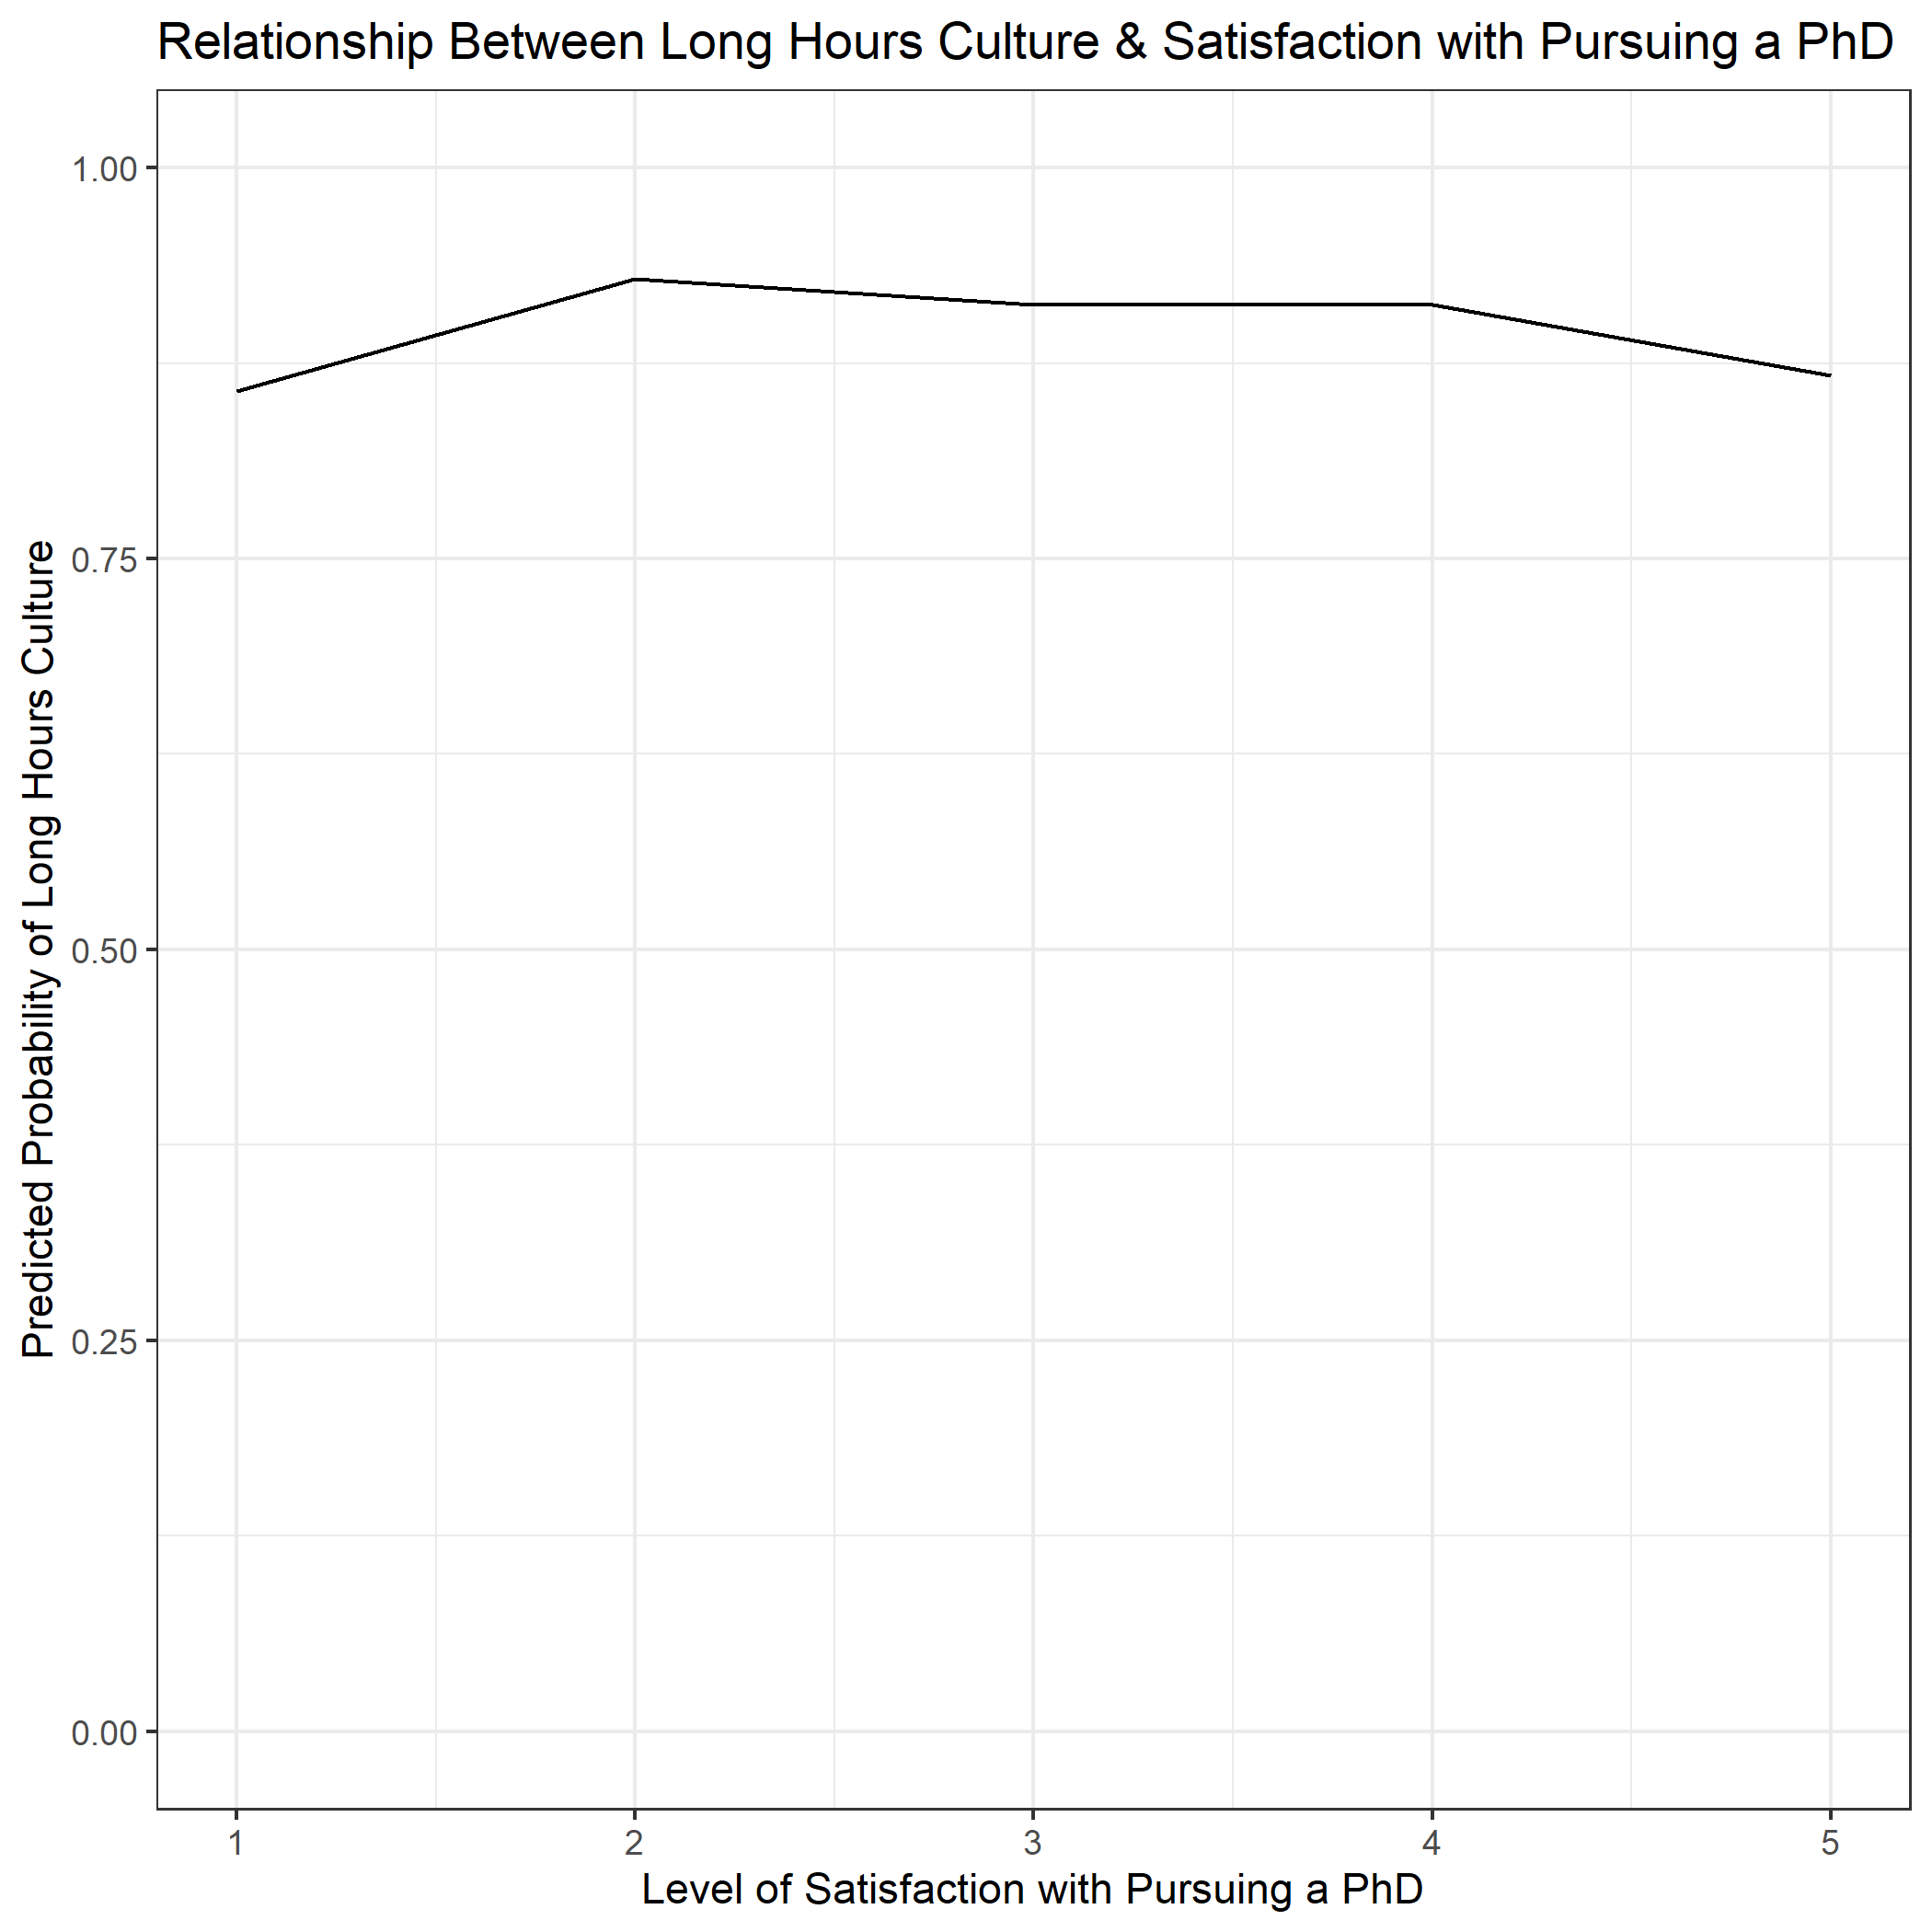
\includegraphics[width=29.17in]{C:/Users/iciar/OneDrive/Desktop/School/STAT547/group05/images/logisticregression}

\hypertarget{lr2-supervisor-relationship-phd-satisfaction}{%
\paragraph{LR2: Supervisor Relationship \textasciitilde{} PhD
Satisfaction}\label{lr2-supervisor-relationship-phd-satisfaction}}

\begin{Shaded}
\begin{Highlighting}[]
\NormalTok{knitr}\OperatorTok{::}\KeywordTok{include_graphics}\NormalTok{(here}\OperatorTok{::}\KeywordTok{here}\NormalTok{(}\StringTok{"images"}\NormalTok{, }\StringTok{"logisticregression2.png"}\NormalTok{), }\DataTypeTok{auto_pdf =} \KeywordTok{getOption}\NormalTok{(}\StringTok{"knitr.graphics.auto_pdf"}\NormalTok{, }\OtherTok{FALSE}\NormalTok{), }
    \DataTypeTok{dpi =} \OtherTok{NULL}\NormalTok{)}
\end{Highlighting}
\end{Shaded}

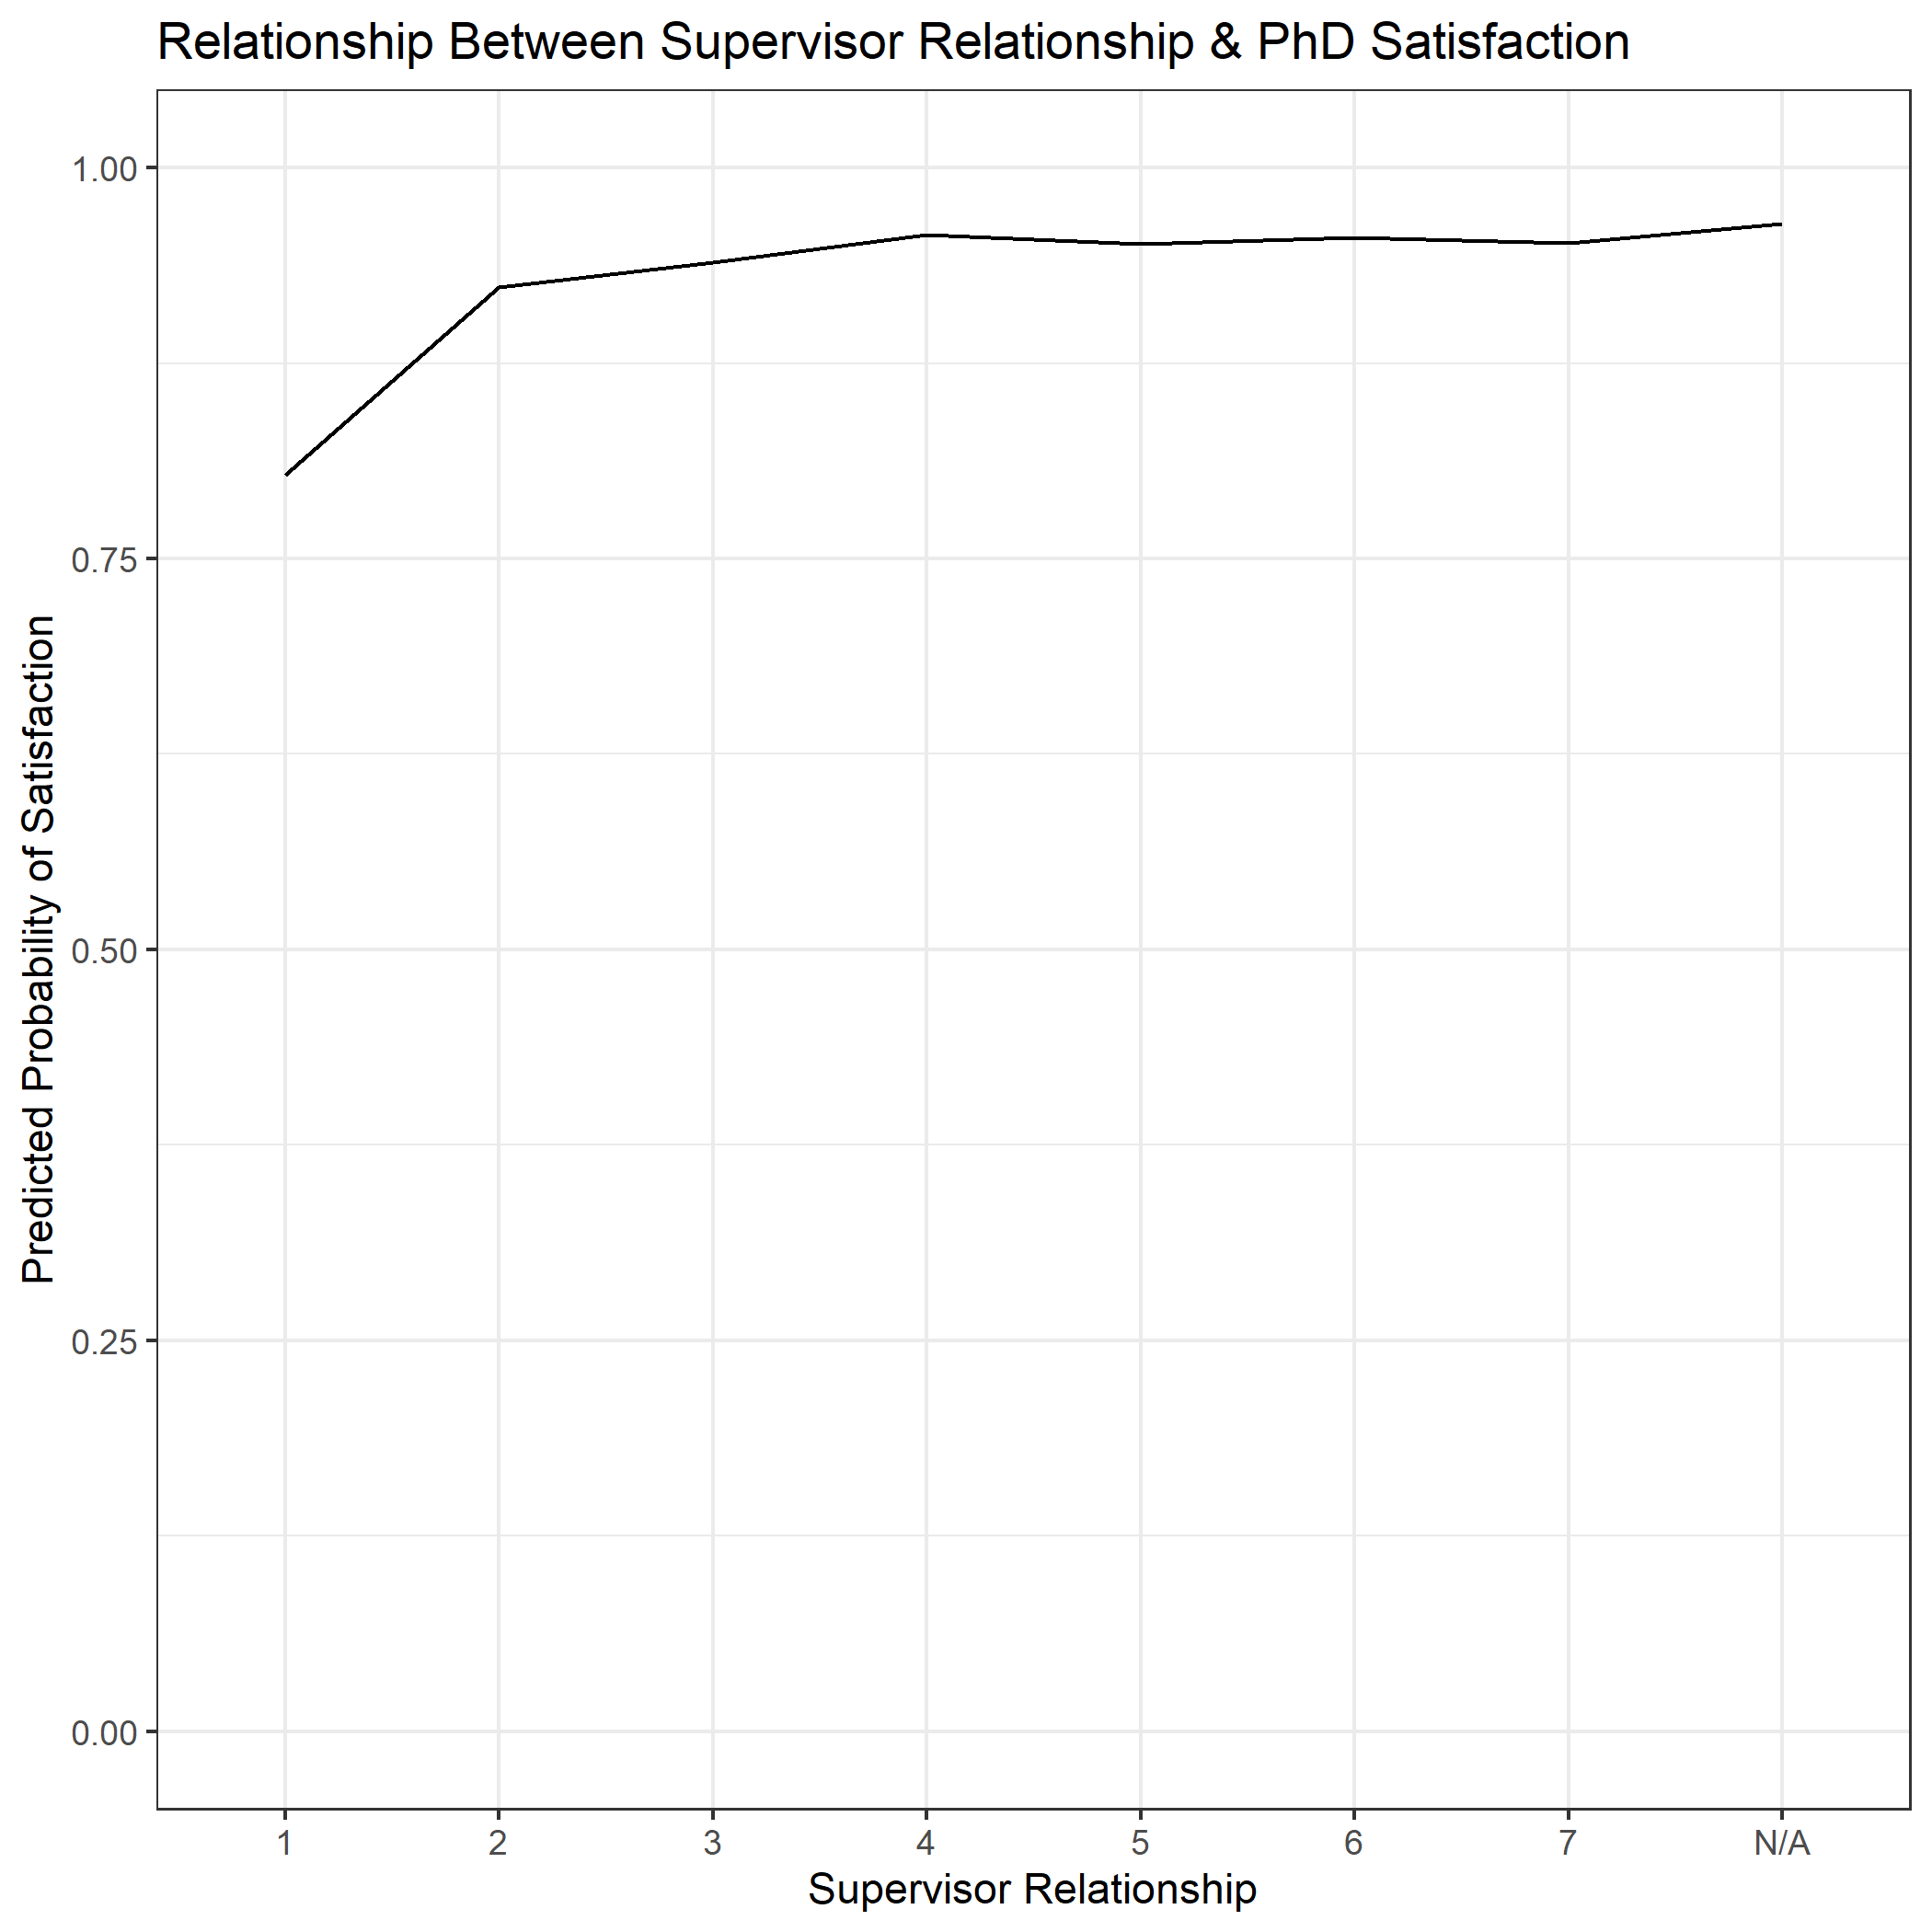
\includegraphics[width=29.17in]{C:/Users/iciar/OneDrive/Desktop/School/STAT547/group05/images/logisticregression2}

\begin{Shaded}
\begin{Highlighting}[]
\NormalTok{knitr}\OperatorTok{::}\KeywordTok{include_graphics}\NormalTok{(here}\OperatorTok{::}\KeywordTok{here}\NormalTok{(}\StringTok{"images"}\NormalTok{, }\StringTok{"satisfaction_v_supervis_relationship.png"}\NormalTok{), }\DataTypeTok{auto_pdf =} \KeywordTok{getOption}\NormalTok{(}\StringTok{"knitr.graphics.auto_pdf"}\NormalTok{, }\OtherTok{FALSE}\NormalTok{), }
    \DataTypeTok{dpi =} \OtherTok{NULL}\NormalTok{)}
\end{Highlighting}
\end{Shaded}

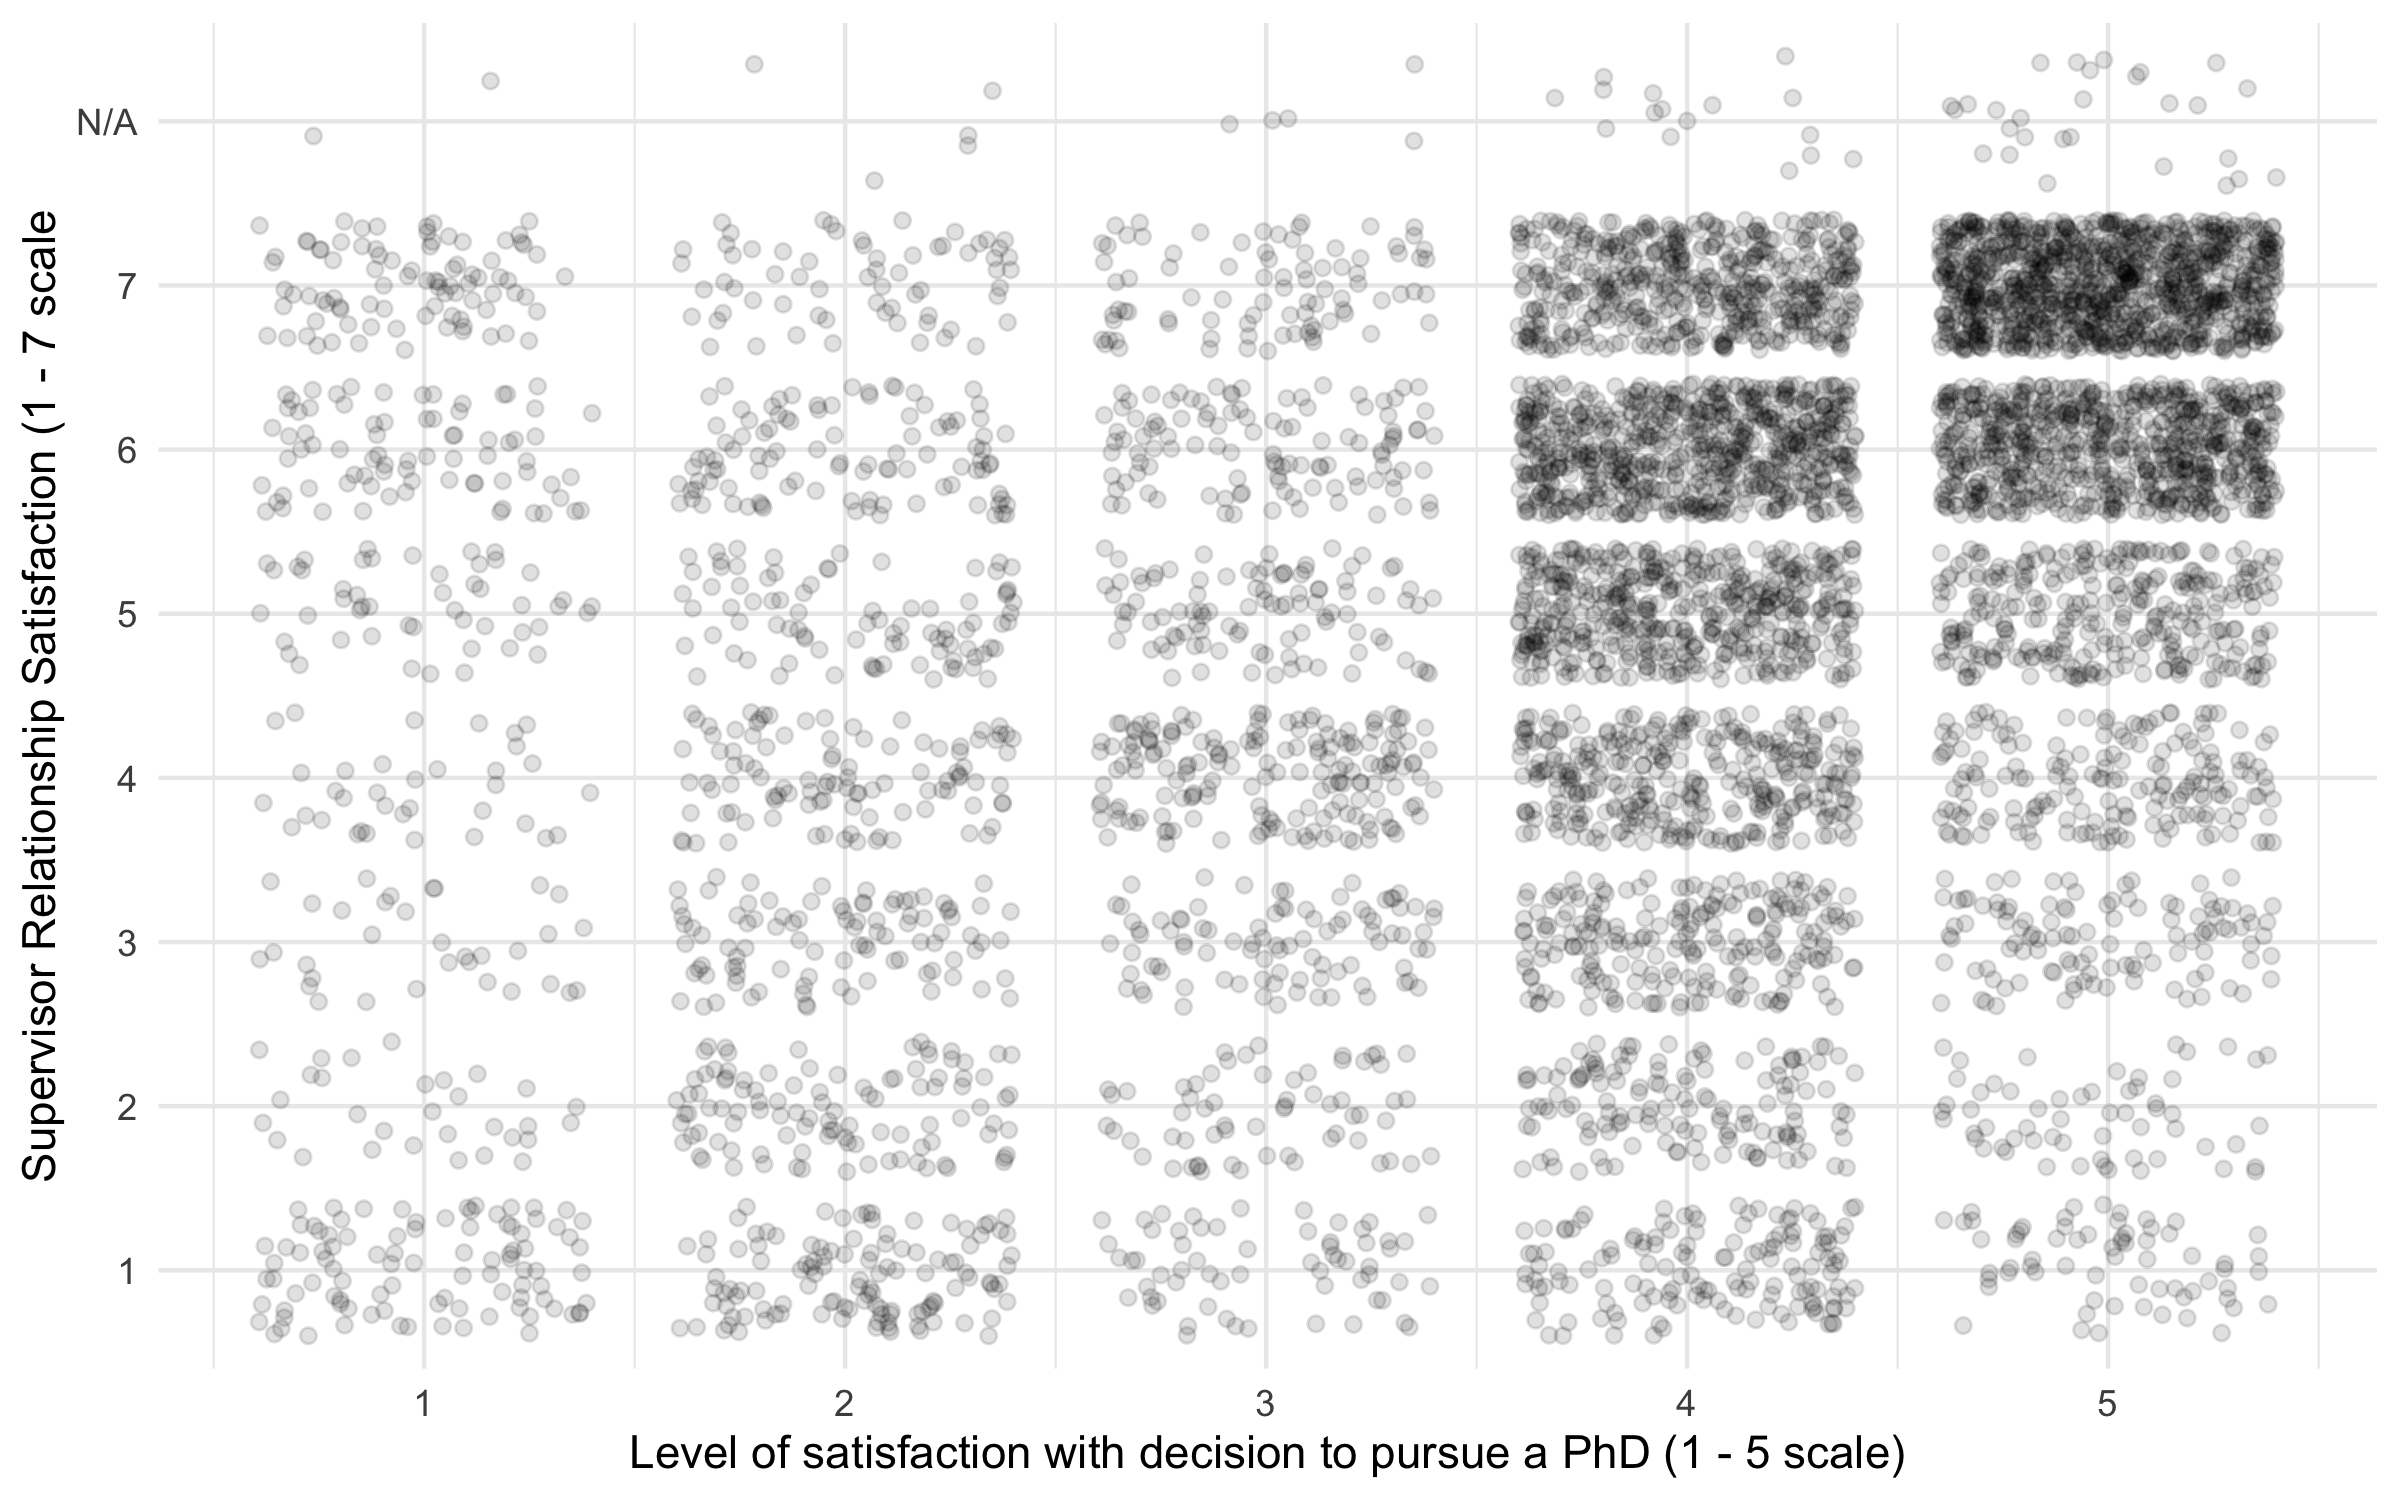
\includegraphics[width=33.33in]{C:/Users/iciar/OneDrive/Desktop/School/STAT547/group05/images/satisfaction_v_supervis_relationship}

\hypertarget{lr3-worklife-balance-phd-satisfaction}{%
\paragraph{LR3: Work/Life Balance \textasciitilde{} PhD
Satisfaction}\label{lr3-worklife-balance-phd-satisfaction}}

\begin{Shaded}
\begin{Highlighting}[]
\NormalTok{knitr}\OperatorTok{::}\KeywordTok{include_graphics}\NormalTok{(here}\OperatorTok{::}\KeywordTok{here}\NormalTok{(}\StringTok{"images"}\NormalTok{, }\StringTok{"logisticregression5.png"}\NormalTok{), }\DataTypeTok{auto_pdf =} \KeywordTok{getOption}\NormalTok{(}\StringTok{"knitr.graphics.auto_pdf"}\NormalTok{, }\OtherTok{FALSE}\NormalTok{), }
    \DataTypeTok{dpi =} \OtherTok{NULL}\NormalTok{)}
\end{Highlighting}
\end{Shaded}

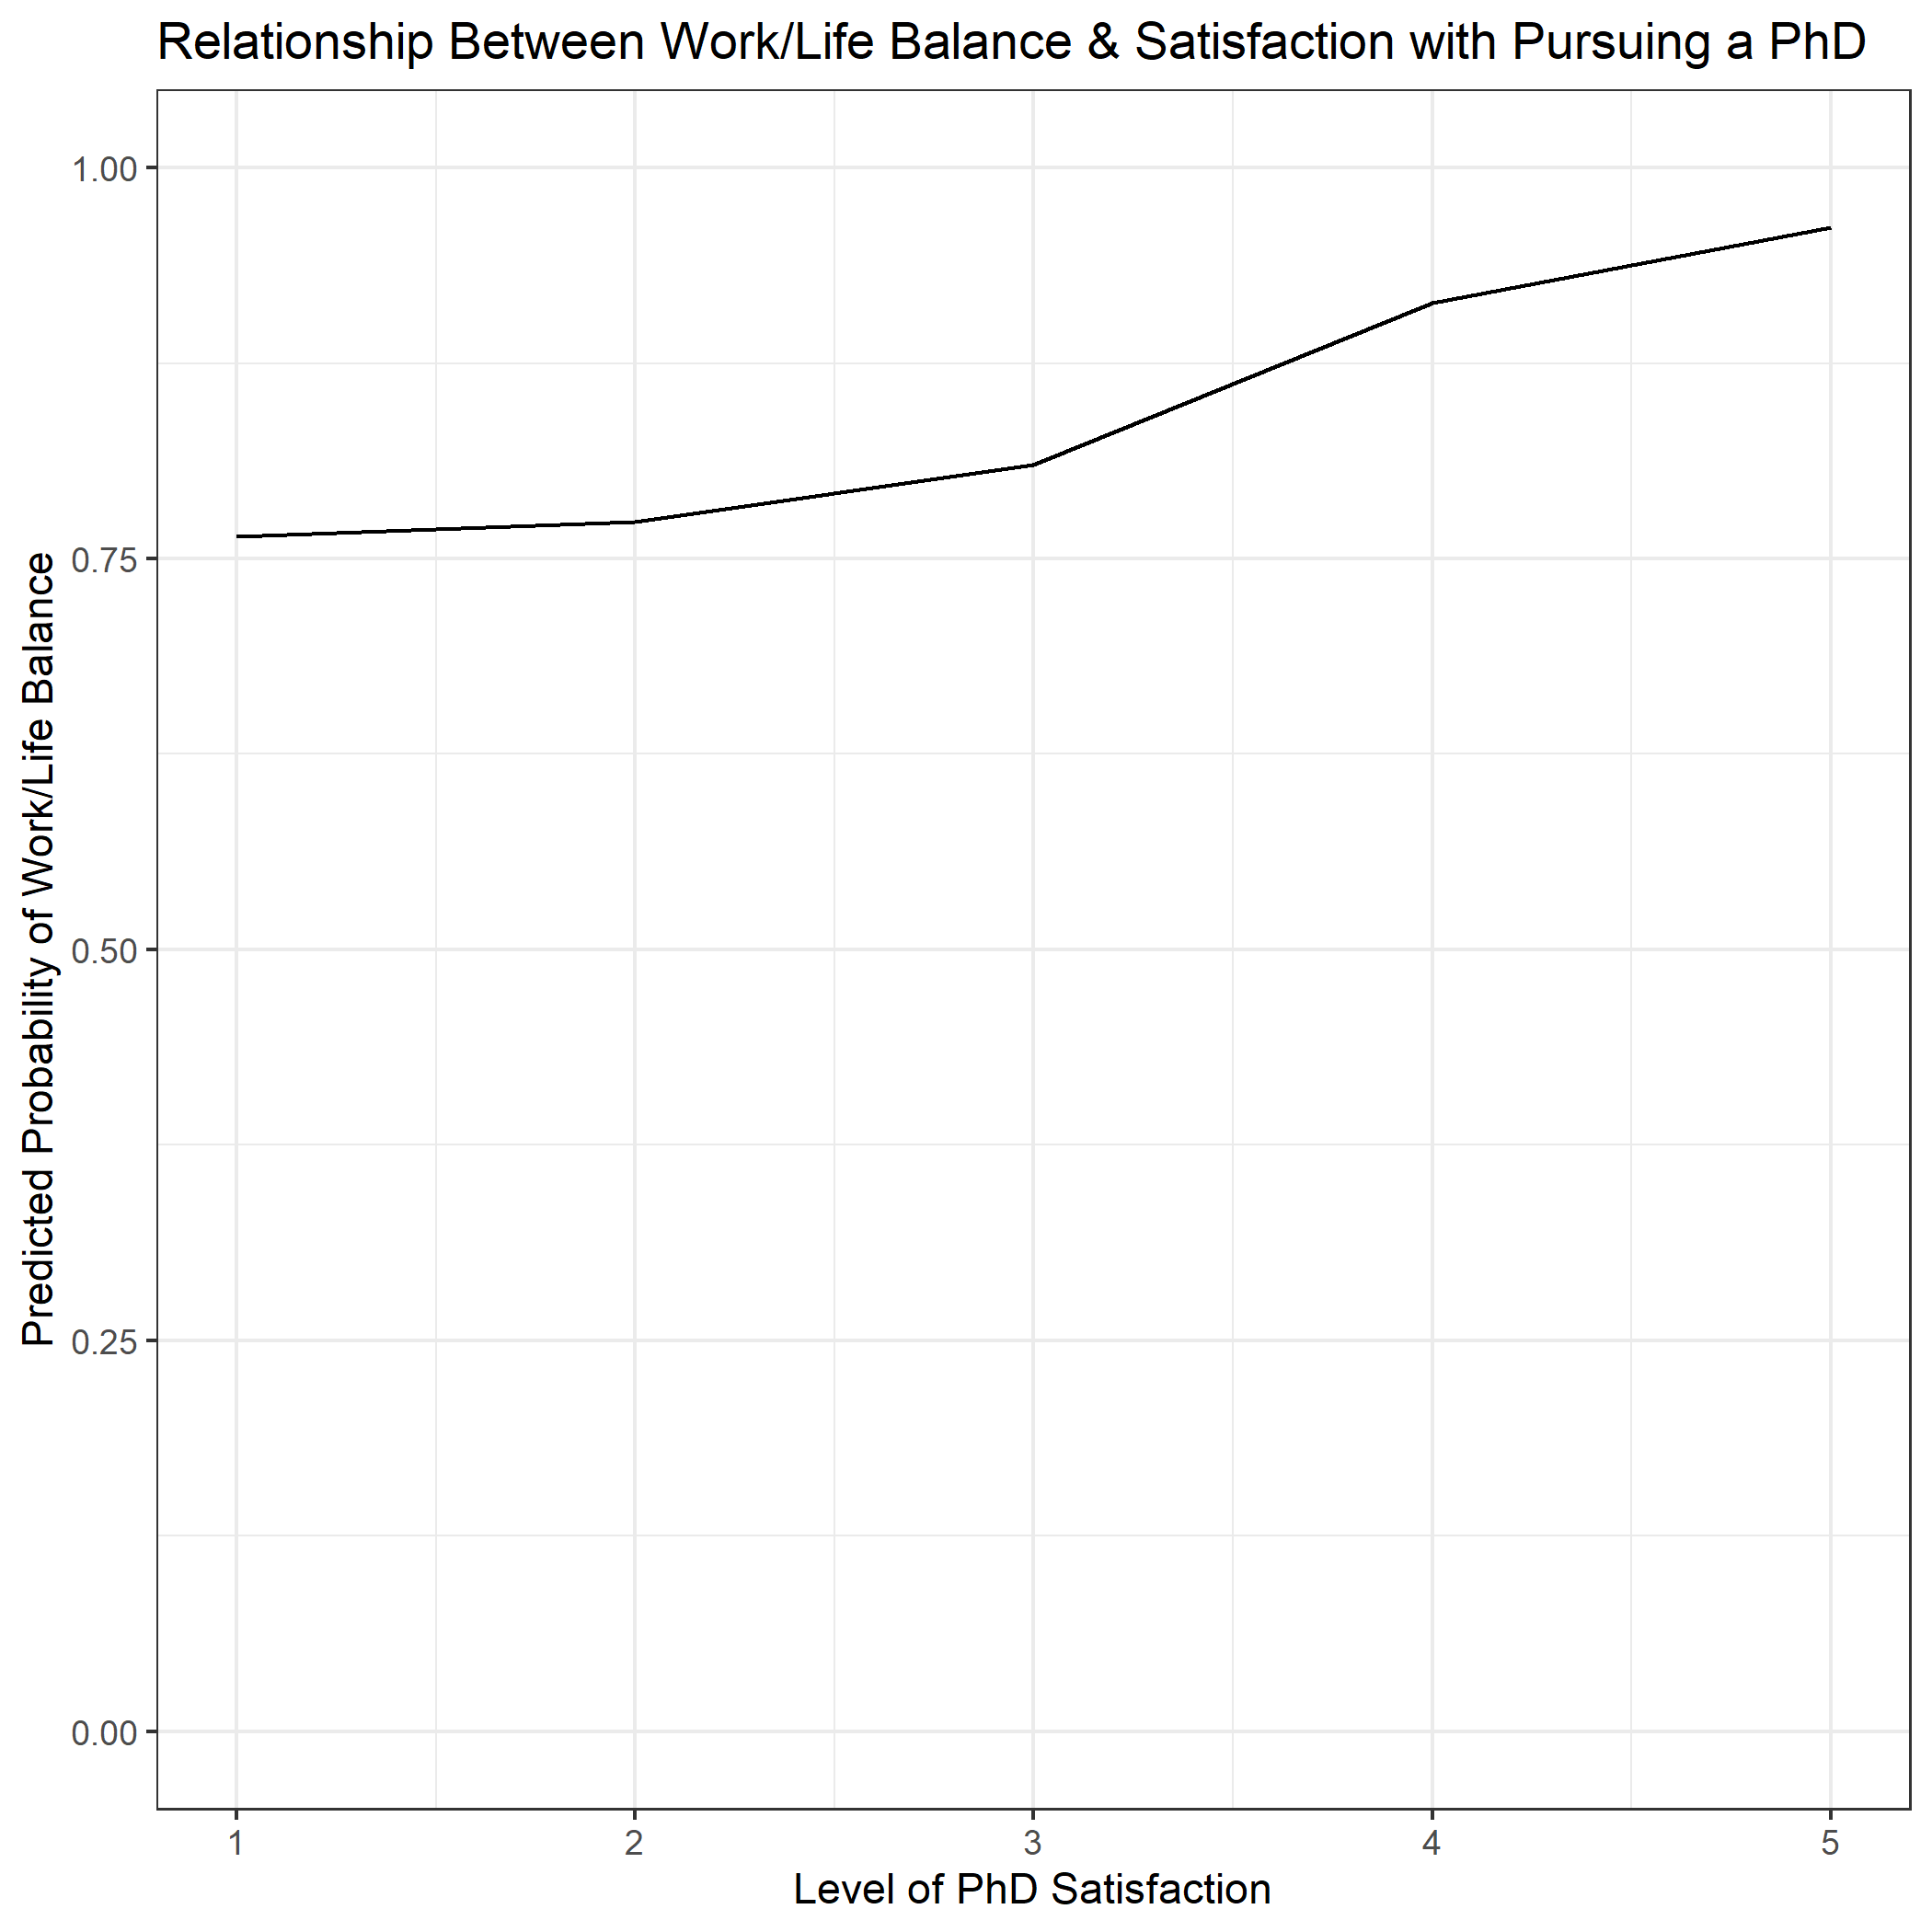
\includegraphics[width=29.17in]{C:/Users/iciar/OneDrive/Desktop/School/STAT547/group05/images/logisticregression5}

\begin{Shaded}
\begin{Highlighting}[]
\NormalTok{knitr}\OperatorTok{::}\KeywordTok{include_graphics}\NormalTok{(here}\OperatorTok{::}\KeywordTok{here}\NormalTok{(}\StringTok{"images"}\NormalTok{, }\StringTok{"satisfaction_v_work_life_bal.png"}\NormalTok{), }\DataTypeTok{auto_pdf =} \KeywordTok{getOption}\NormalTok{(}\StringTok{"knitr.graphics.auto_pdf"}\NormalTok{, }\OtherTok{FALSE}\NormalTok{), }
    \DataTypeTok{dpi =} \OtherTok{NULL}\NormalTok{)}
\end{Highlighting}
\end{Shaded}

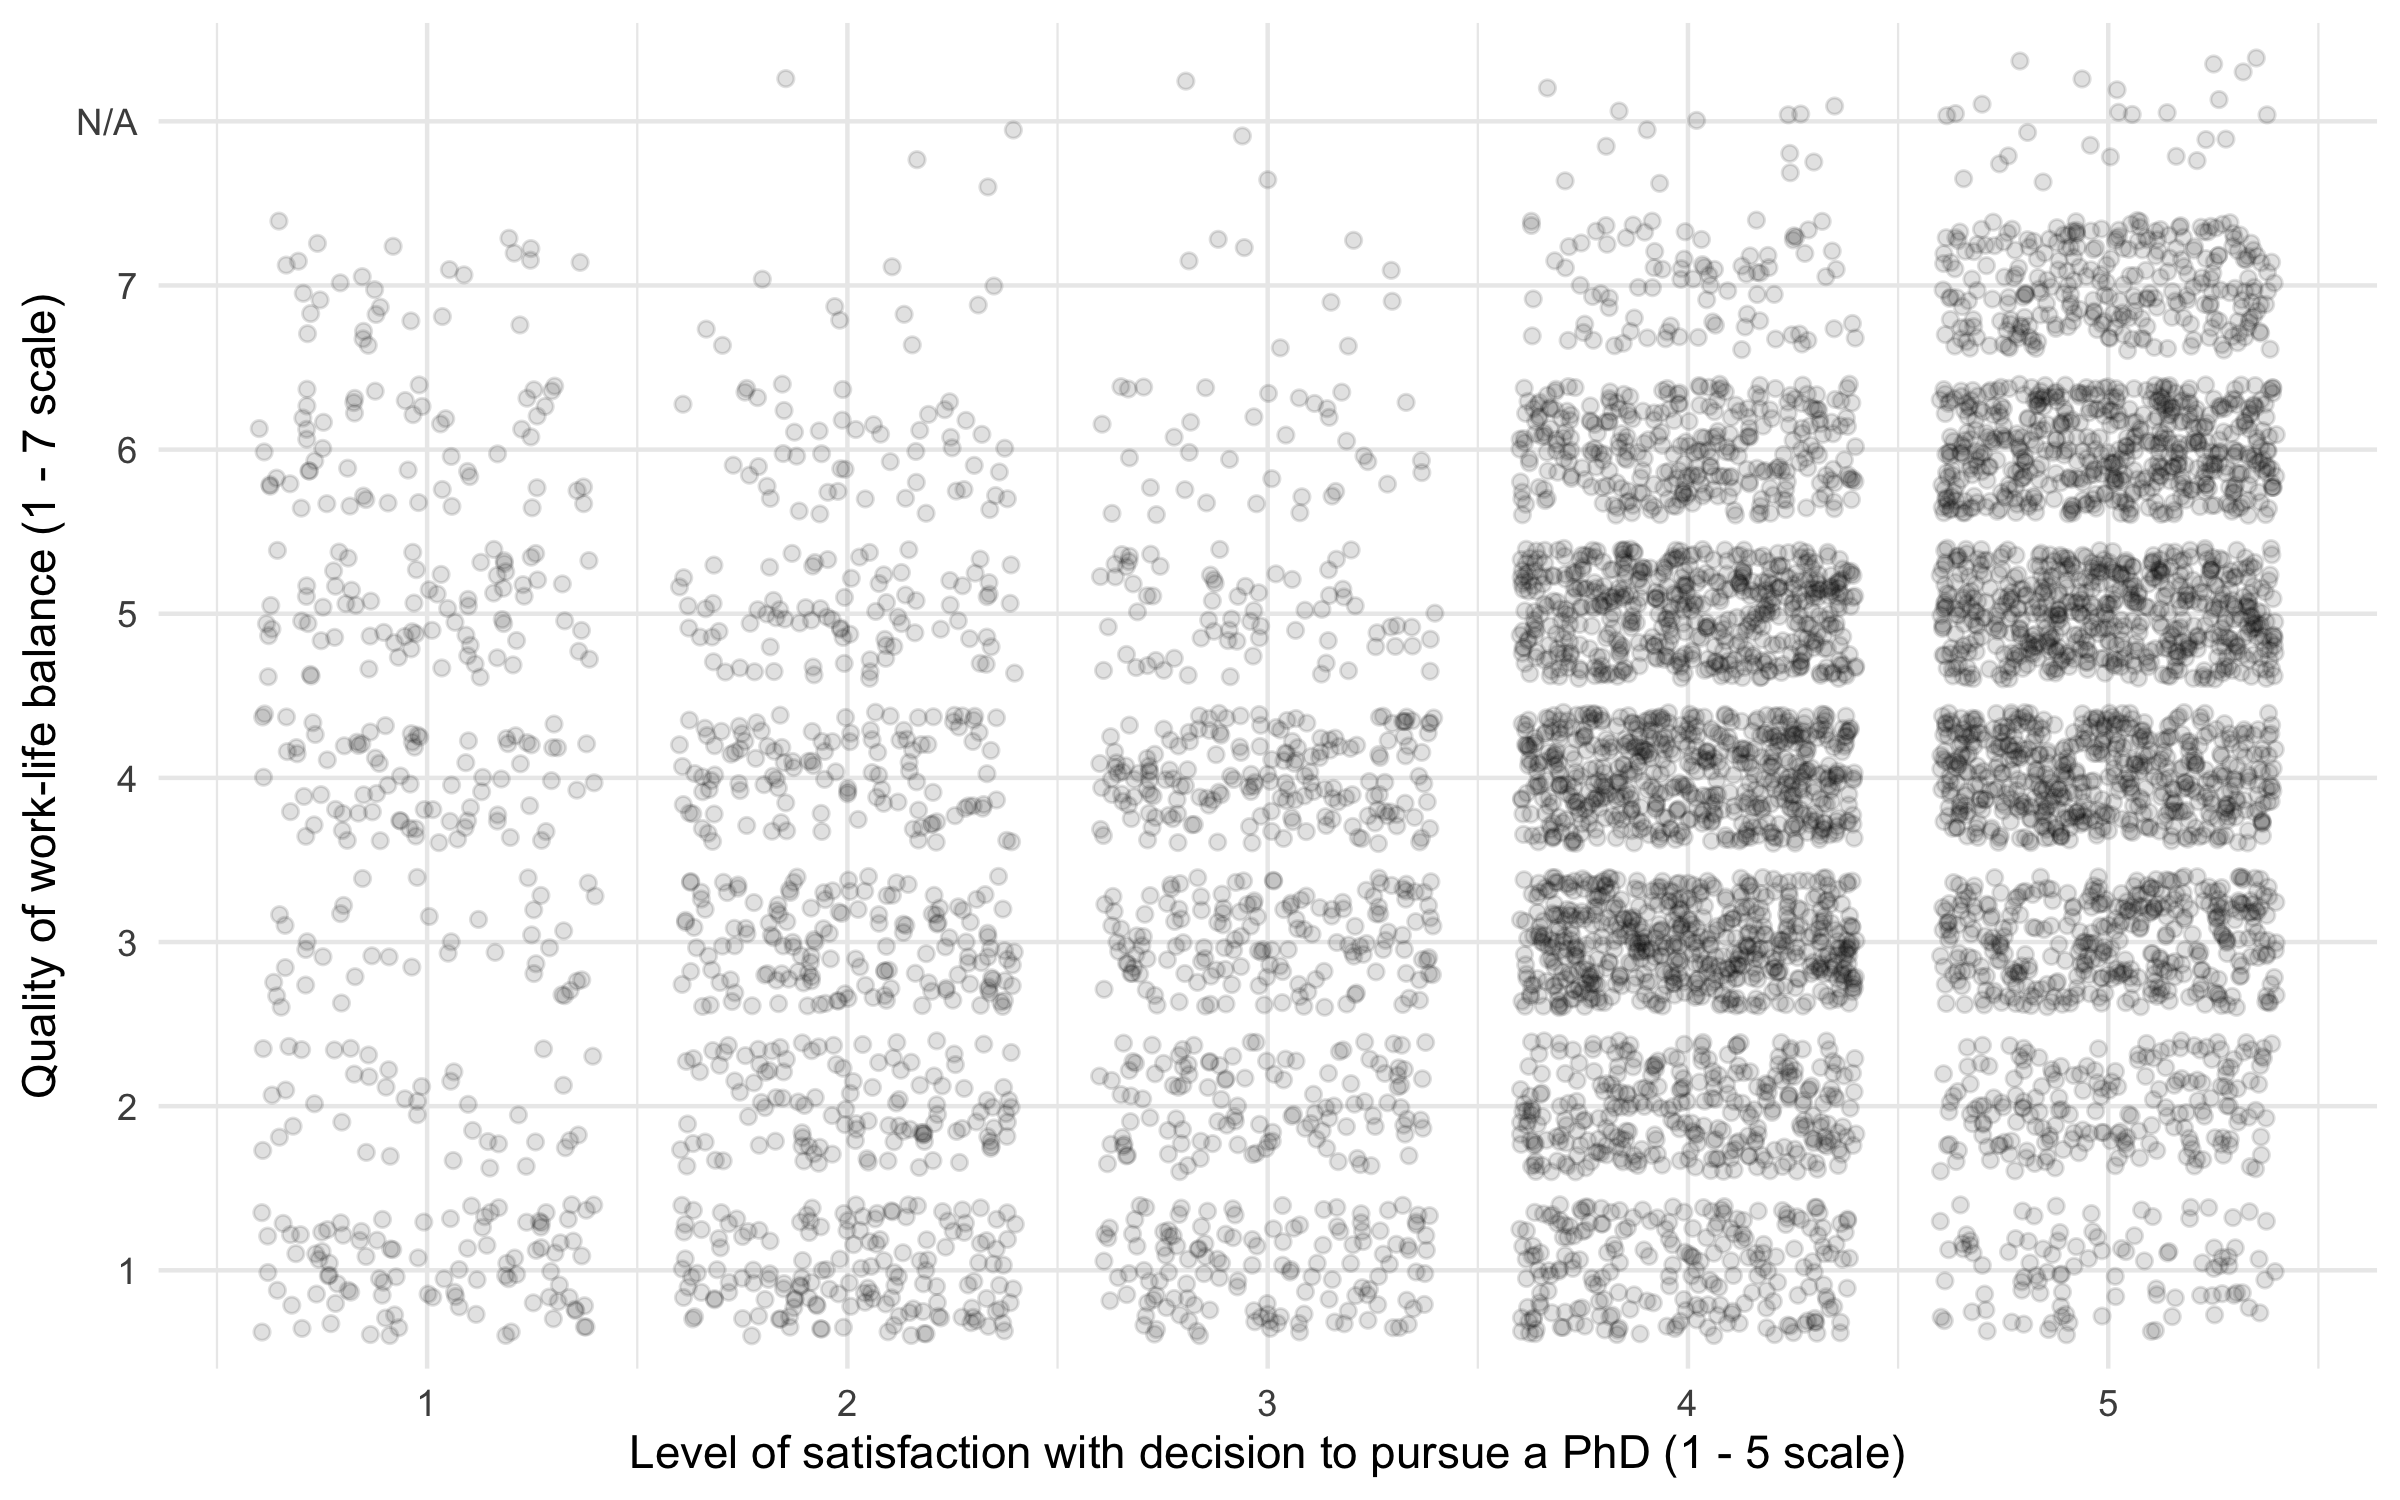
\includegraphics[width=33.33in]{C:/Users/iciar/OneDrive/Desktop/School/STAT547/group05/images/satisfaction_v_work_life_bal}

\hypertarget{lr4-supervisor-relationship-anxiety-or-depression}{%
\paragraph{LR4: Supervisor Relationship \textasciitilde{} Anxiety or
Depression}\label{lr4-supervisor-relationship-anxiety-or-depression}}

\begin{Shaded}
\begin{Highlighting}[]
\NormalTok{knitr}\OperatorTok{::}\KeywordTok{include_graphics}\NormalTok{(here}\OperatorTok{::}\KeywordTok{here}\NormalTok{(}\StringTok{"images"}\NormalTok{, }\StringTok{"logisticregression3.png"}\NormalTok{), }\DataTypeTok{auto_pdf =} \KeywordTok{getOption}\NormalTok{(}\StringTok{"knitr.graphics.auto_pdf"}\NormalTok{, }\OtherTok{FALSE}\NormalTok{), }
    \DataTypeTok{dpi =} \OtherTok{NULL}\NormalTok{)}
\end{Highlighting}
\end{Shaded}

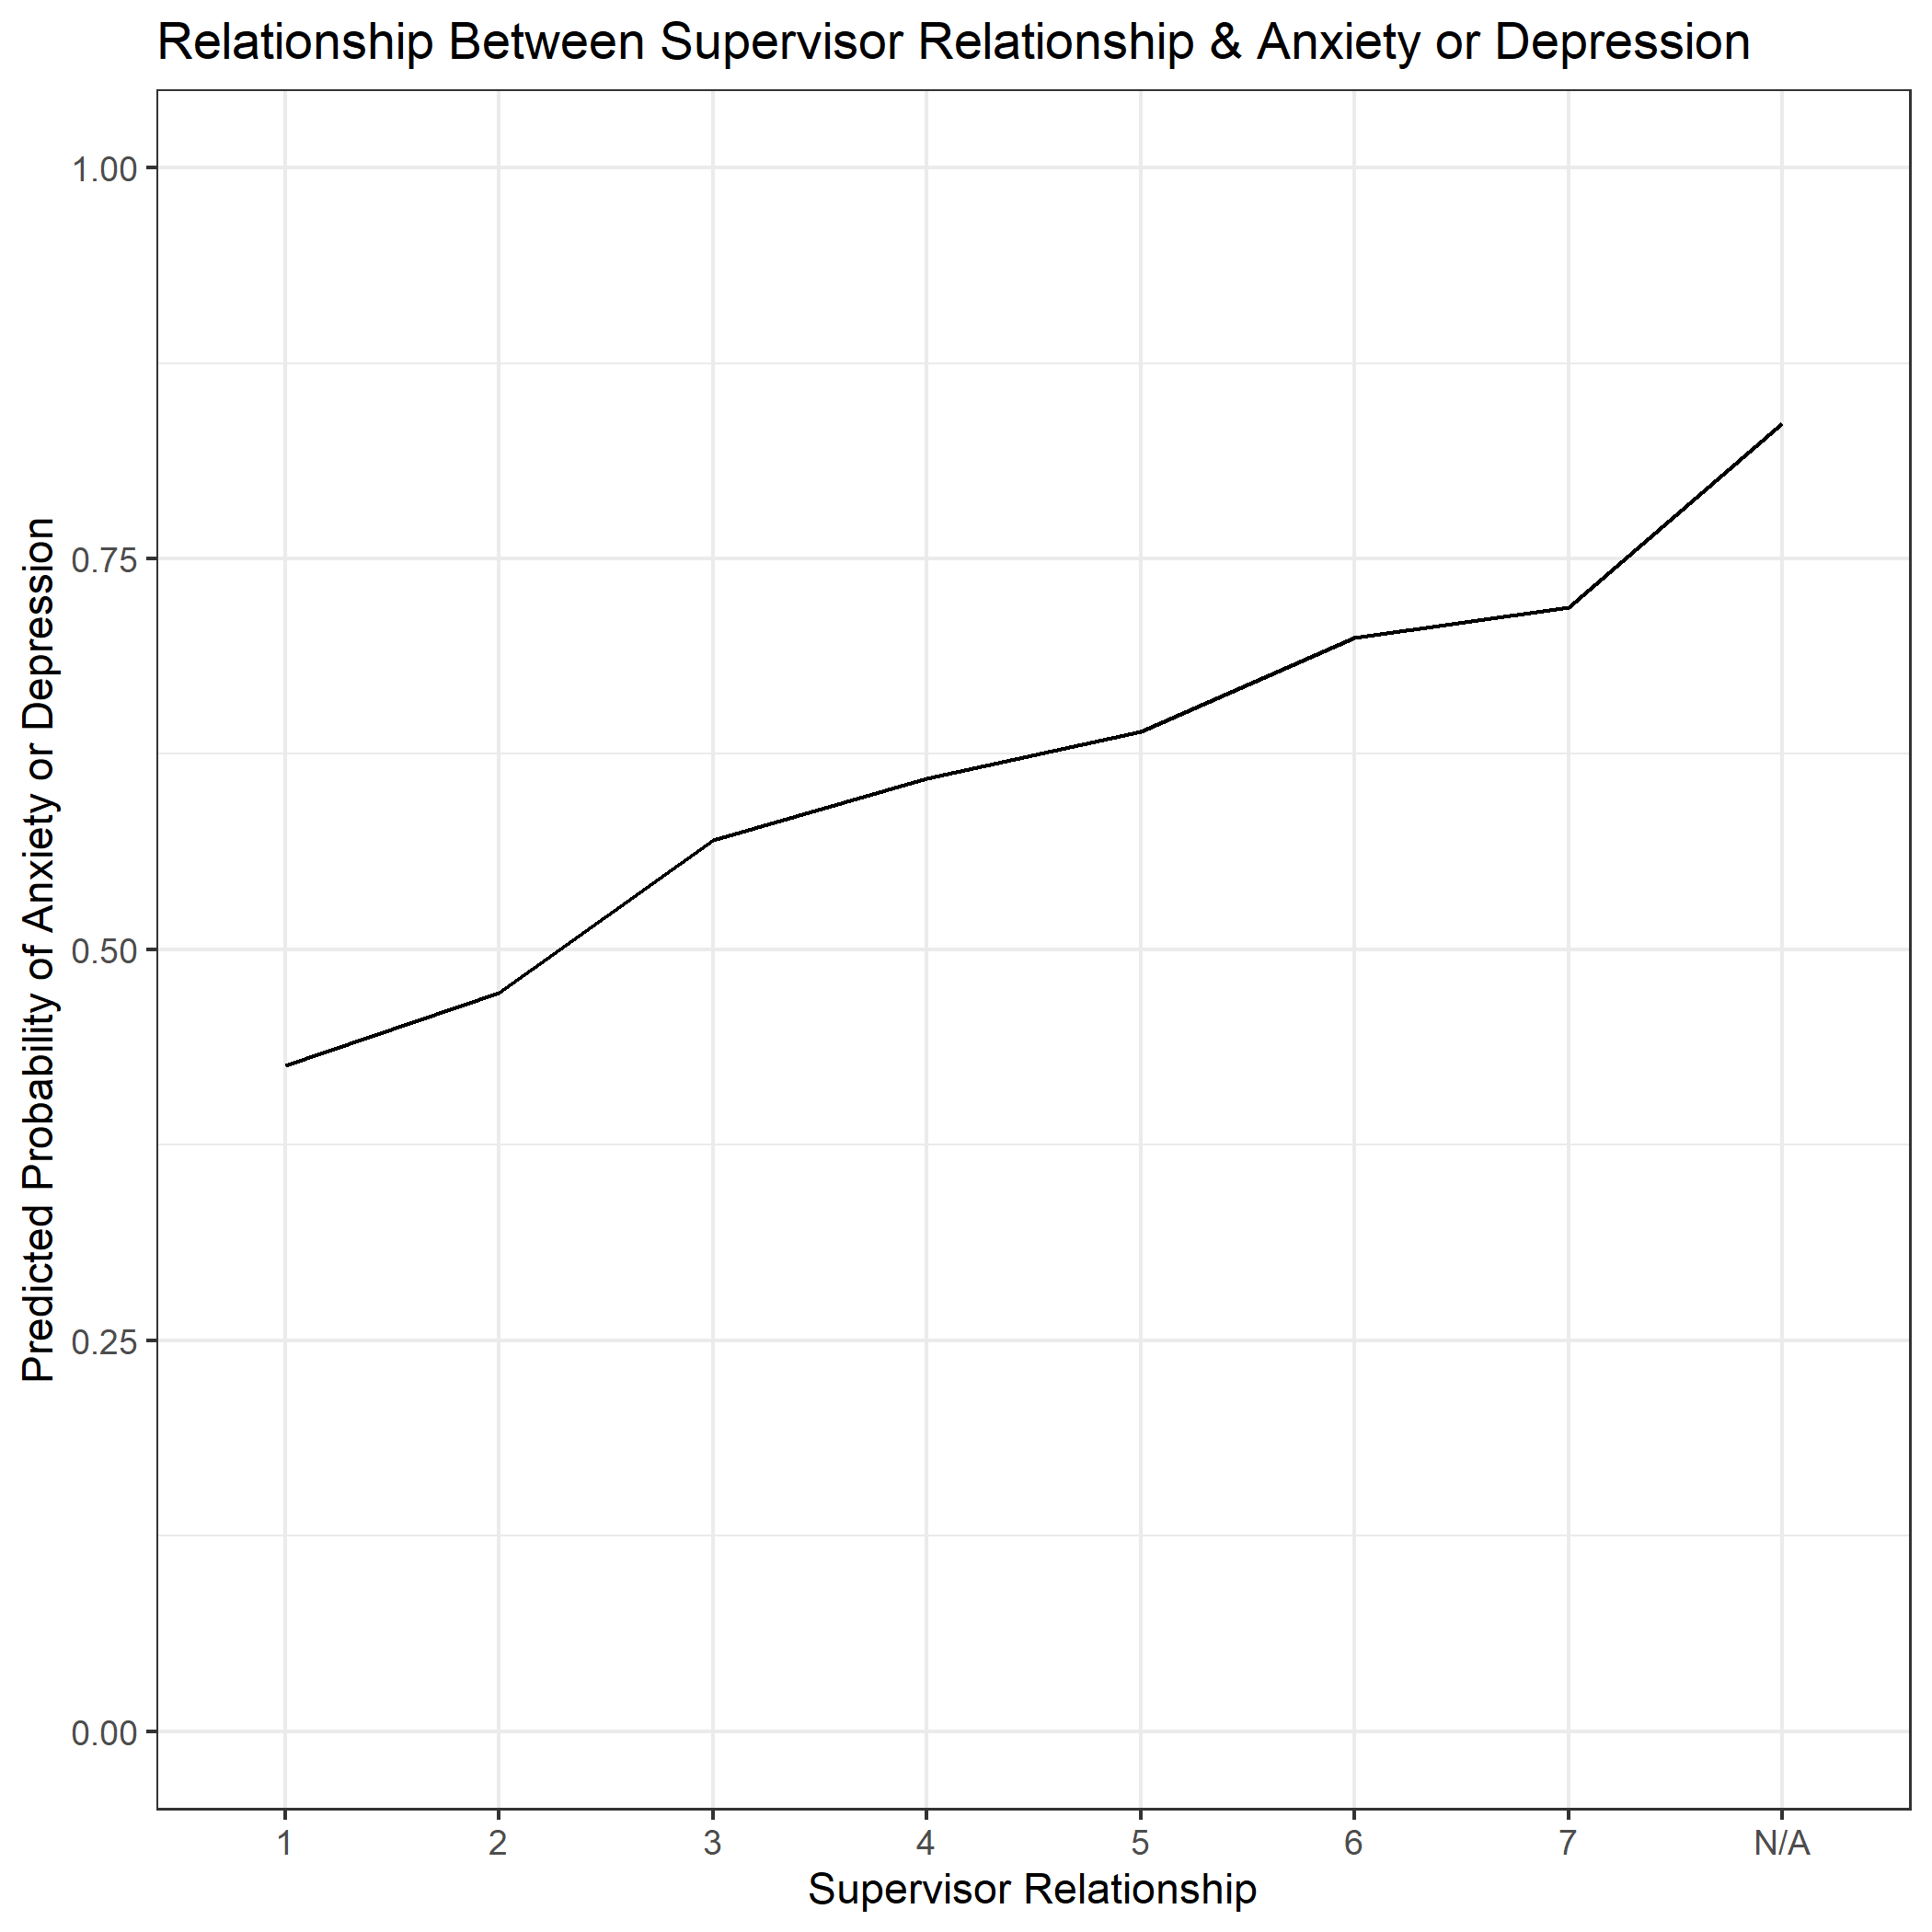
\includegraphics[width=29.17in]{C:/Users/iciar/OneDrive/Desktop/School/STAT547/group05/images/logisticregression3}

\hypertarget{lr5-studying-outside-of-your-home-country-anxiety-or-depression}{%
\paragraph{LR5: Studying Outside of your Home Country \textasciitilde{}
Anxiety or
Depression}\label{lr5-studying-outside-of-your-home-country-anxiety-or-depression}}

\begin{Shaded}
\begin{Highlighting}[]
\NormalTok{knitr}\OperatorTok{::}\KeywordTok{include_graphics}\NormalTok{(here}\OperatorTok{::}\KeywordTok{here}\NormalTok{(}\StringTok{"images"}\NormalTok{, }\StringTok{"logisticregression4.png"}\NormalTok{), }\DataTypeTok{auto_pdf =} \KeywordTok{getOption}\NormalTok{(}\StringTok{"knitr.graphics.auto_pdf"}\NormalTok{, }\OtherTok{FALSE}\NormalTok{), }
    \DataTypeTok{dpi =} \OtherTok{NULL}\NormalTok{)}
\end{Highlighting}
\end{Shaded}

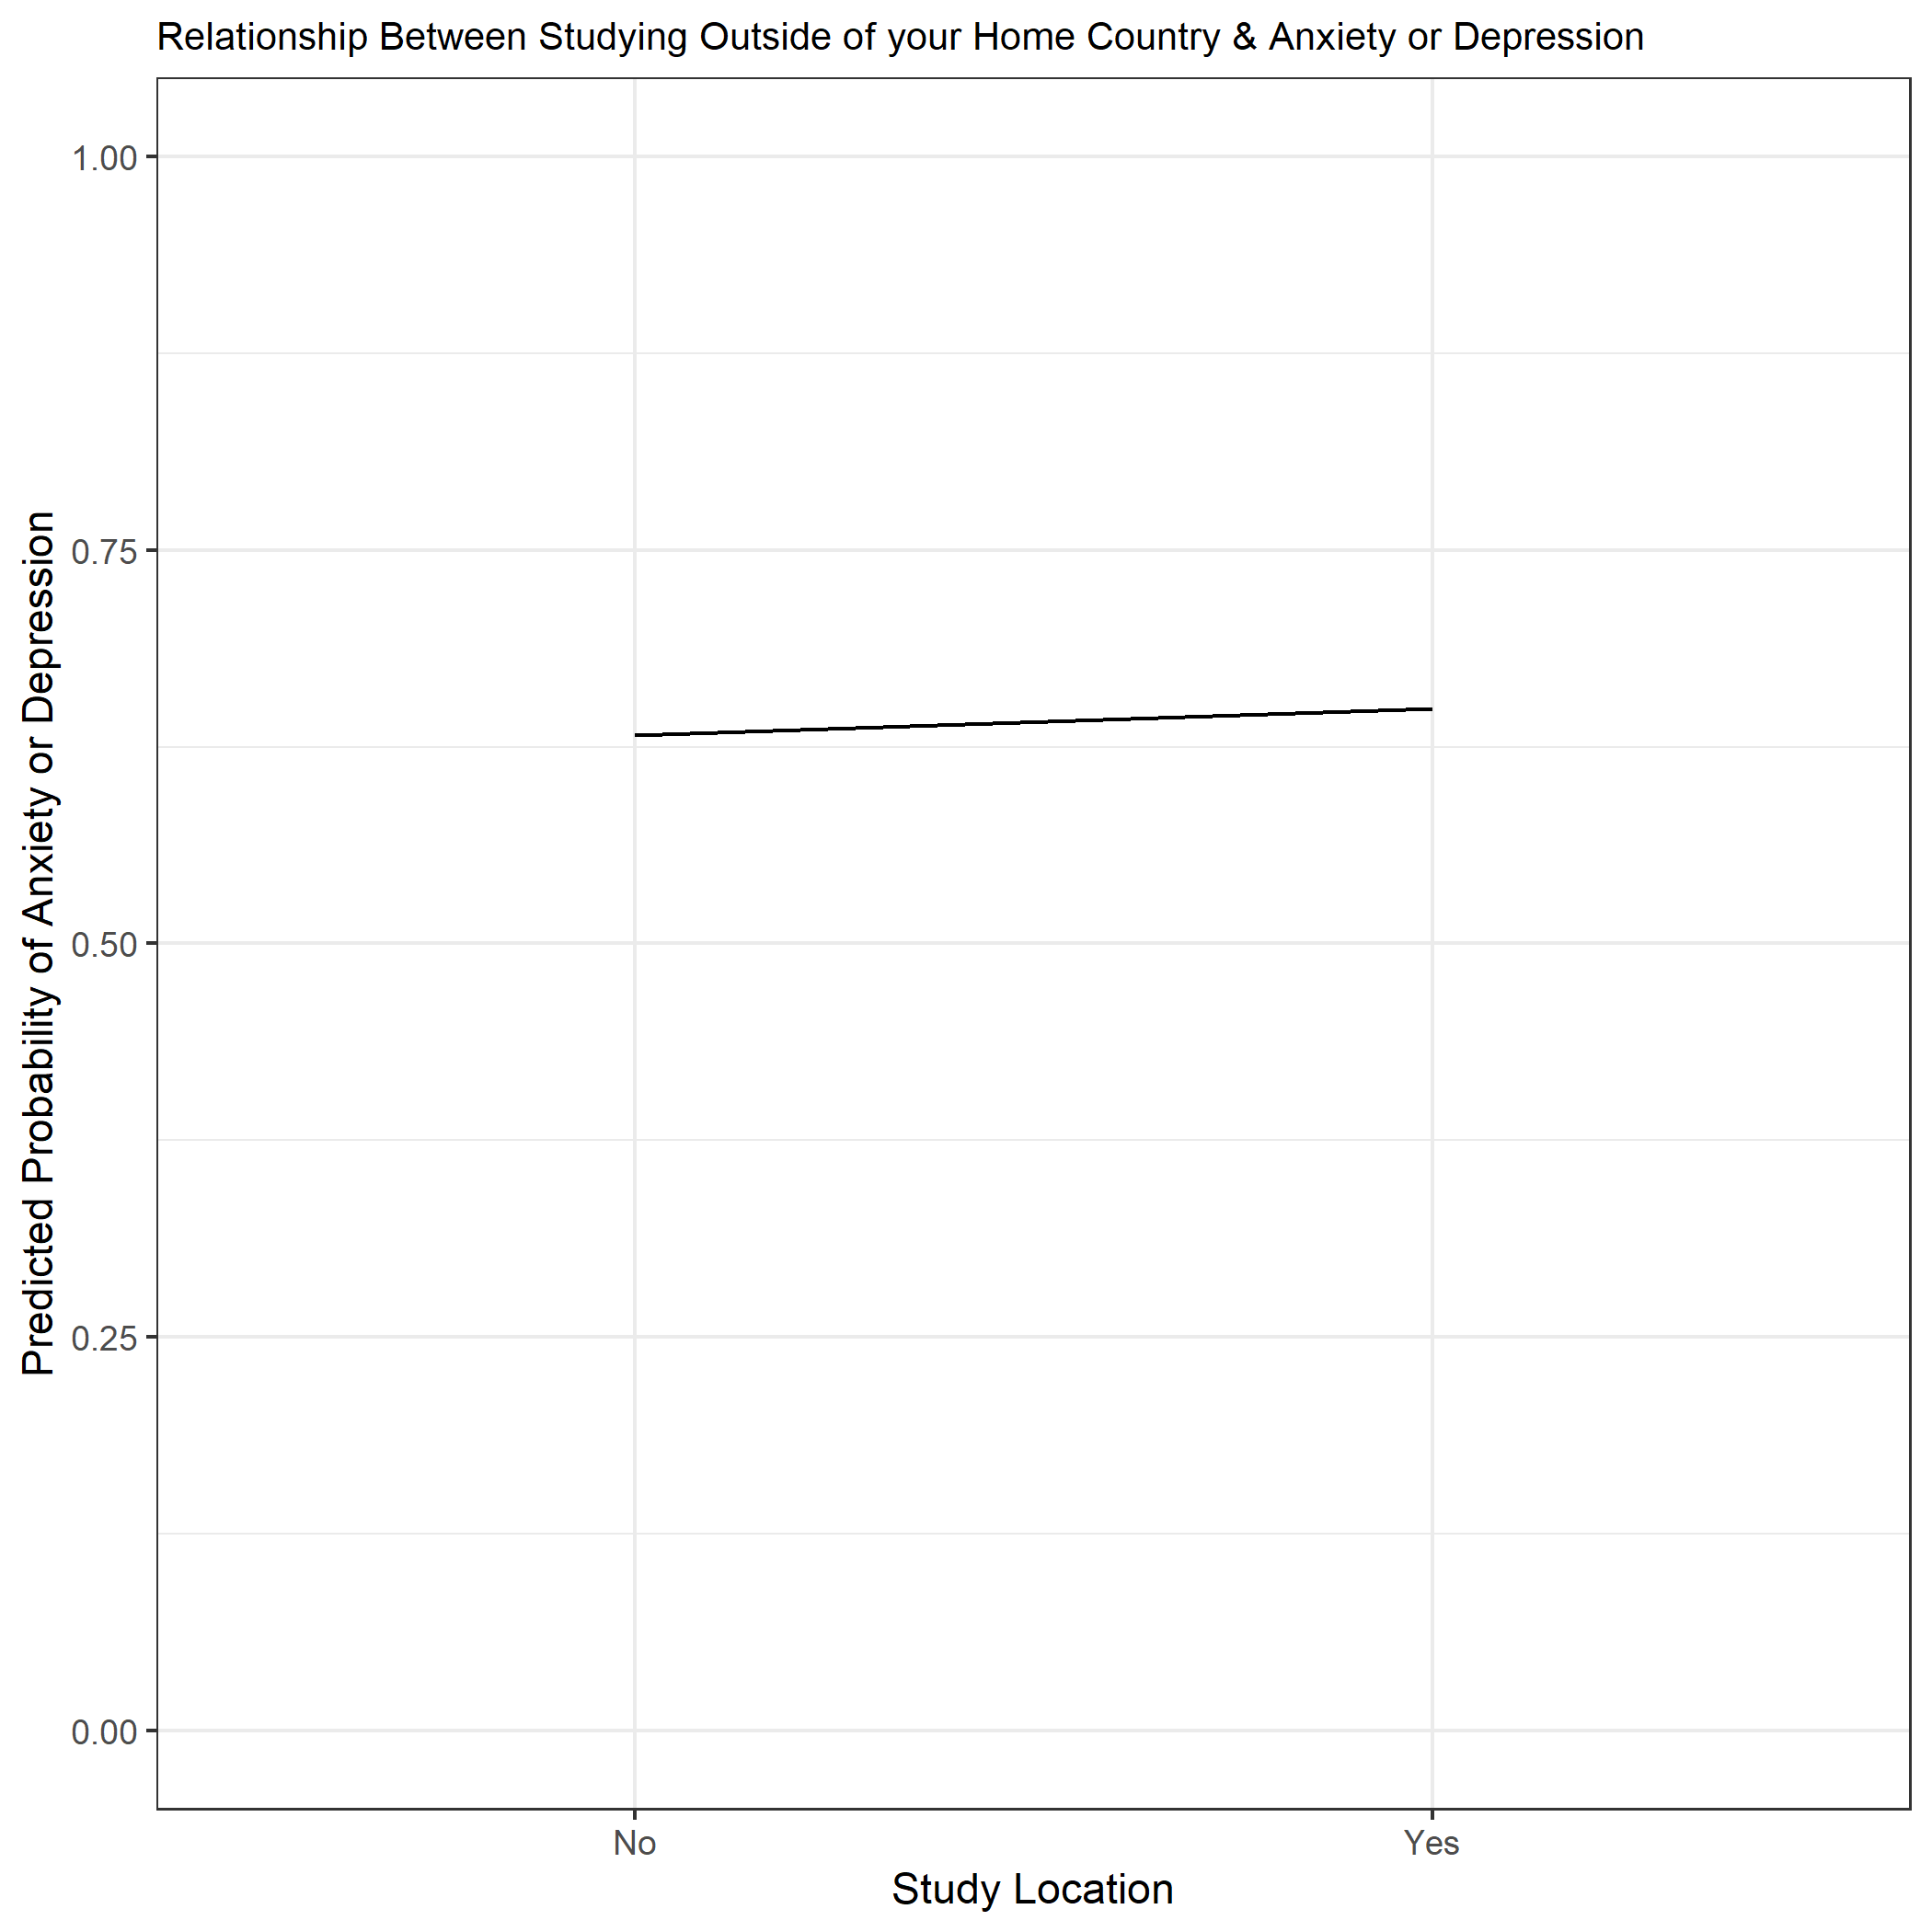
\includegraphics[width=29.17in]{C:/Users/iciar/OneDrive/Desktop/School/STAT547/group05/images/logisticregression4}

\hypertarget{lr6-studying-outside-of-your-home-country-discrimination-or-harrassment}{%
\paragraph{LR6: Studying Outside of your Home Country \textasciitilde{}
Discrimination or
Harrassment}\label{lr6-studying-outside-of-your-home-country-discrimination-or-harrassment}}

\begin{Shaded}
\begin{Highlighting}[]
\NormalTok{knitr}\OperatorTok{::}\KeywordTok{include_graphics}\NormalTok{(here}\OperatorTok{::}\KeywordTok{here}\NormalTok{(}\StringTok{"images"}\NormalTok{, }\StringTok{"logisticregression6.png"}\NormalTok{), }\DataTypeTok{auto_pdf =} \KeywordTok{getOption}\NormalTok{(}\StringTok{"knitr.graphics.auto_pdf"}\NormalTok{, }\OtherTok{FALSE}\NormalTok{), }
    \DataTypeTok{dpi =} \OtherTok{NULL}\NormalTok{)}
\end{Highlighting}
\end{Shaded}

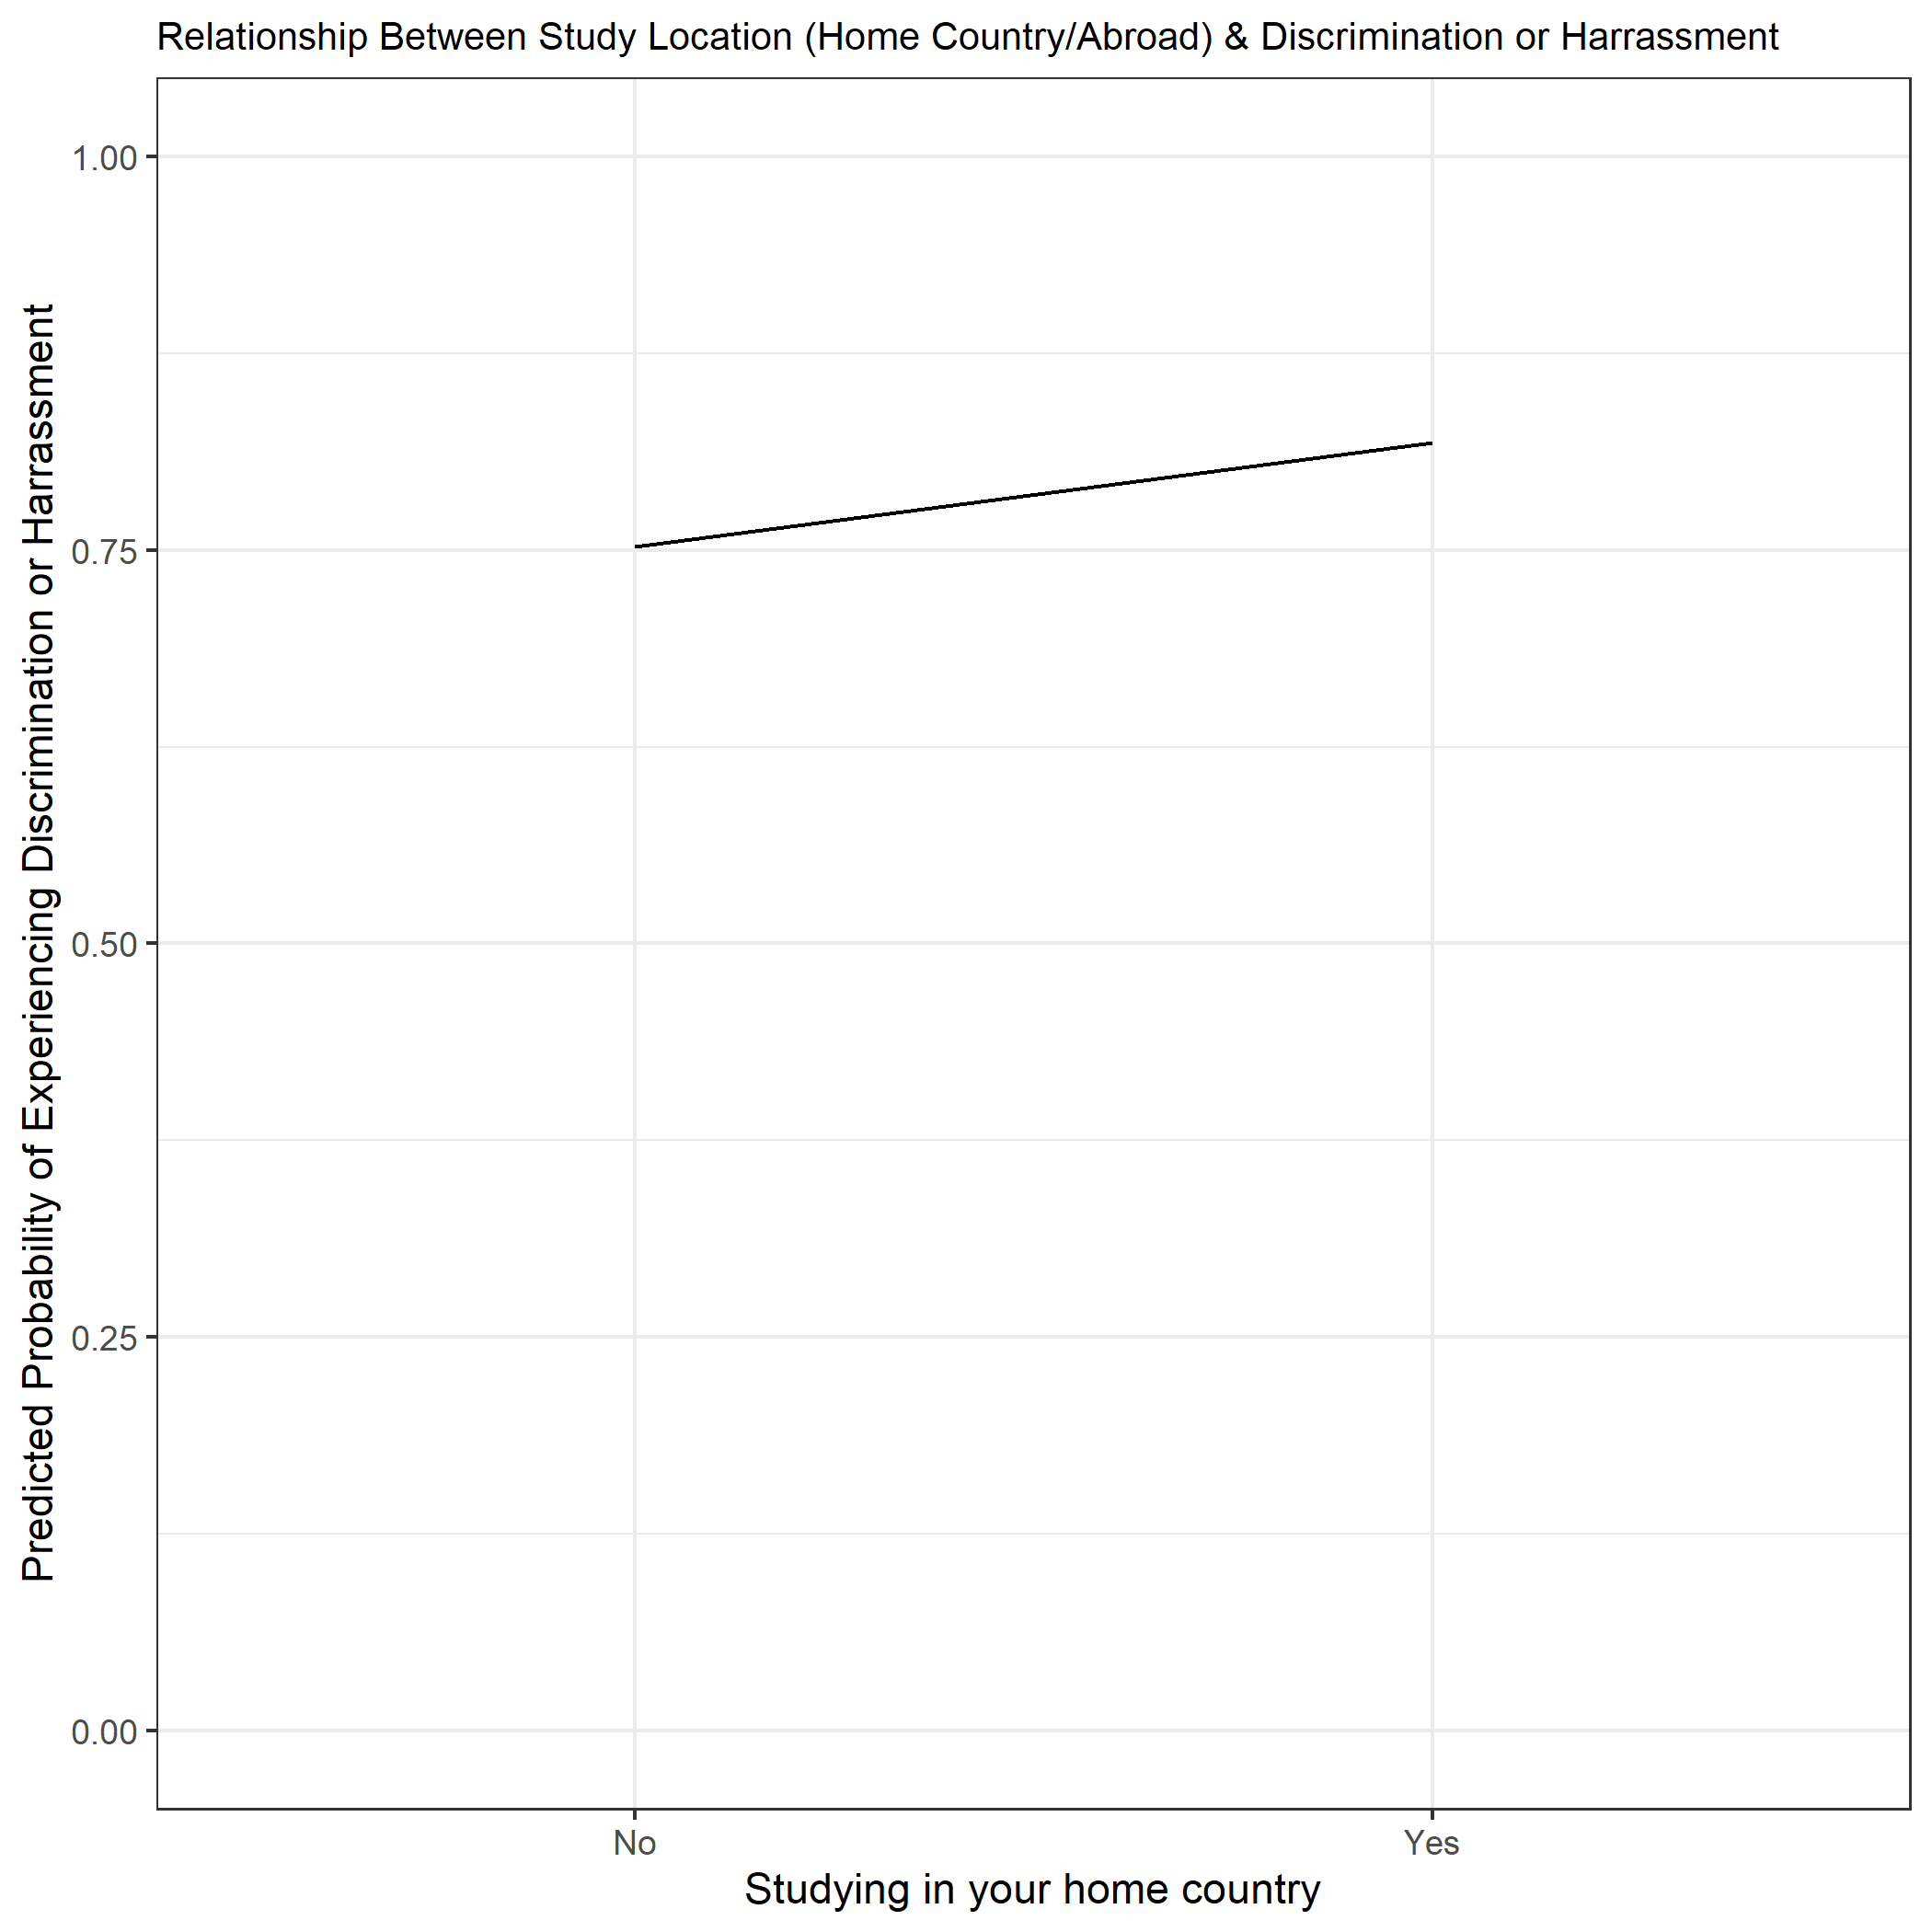
\includegraphics[width=29.17in]{C:/Users/iciar/OneDrive/Desktop/School/STAT547/group05/images/logisticregression6}

\hypertarget{lr7-gender-discrimination-or-harrassment}{%
\paragraph{LR7: Gender \textasciitilde{} Discrimination or
Harrassment}\label{lr7-gender-discrimination-or-harrassment}}

\begin{Shaded}
\begin{Highlighting}[]
\NormalTok{knitr}\OperatorTok{::}\KeywordTok{include_graphics}\NormalTok{(here}\OperatorTok{::}\KeywordTok{here}\NormalTok{(}\StringTok{"images"}\NormalTok{, }\StringTok{"logisticregression7.png"}\NormalTok{), }\DataTypeTok{auto_pdf =} \KeywordTok{getOption}\NormalTok{(}\StringTok{"knitr.graphics.auto_pdf"}\NormalTok{, }\OtherTok{FALSE}\NormalTok{), }
    \DataTypeTok{dpi =} \OtherTok{NULL}\NormalTok{)}
\end{Highlighting}
\end{Shaded}

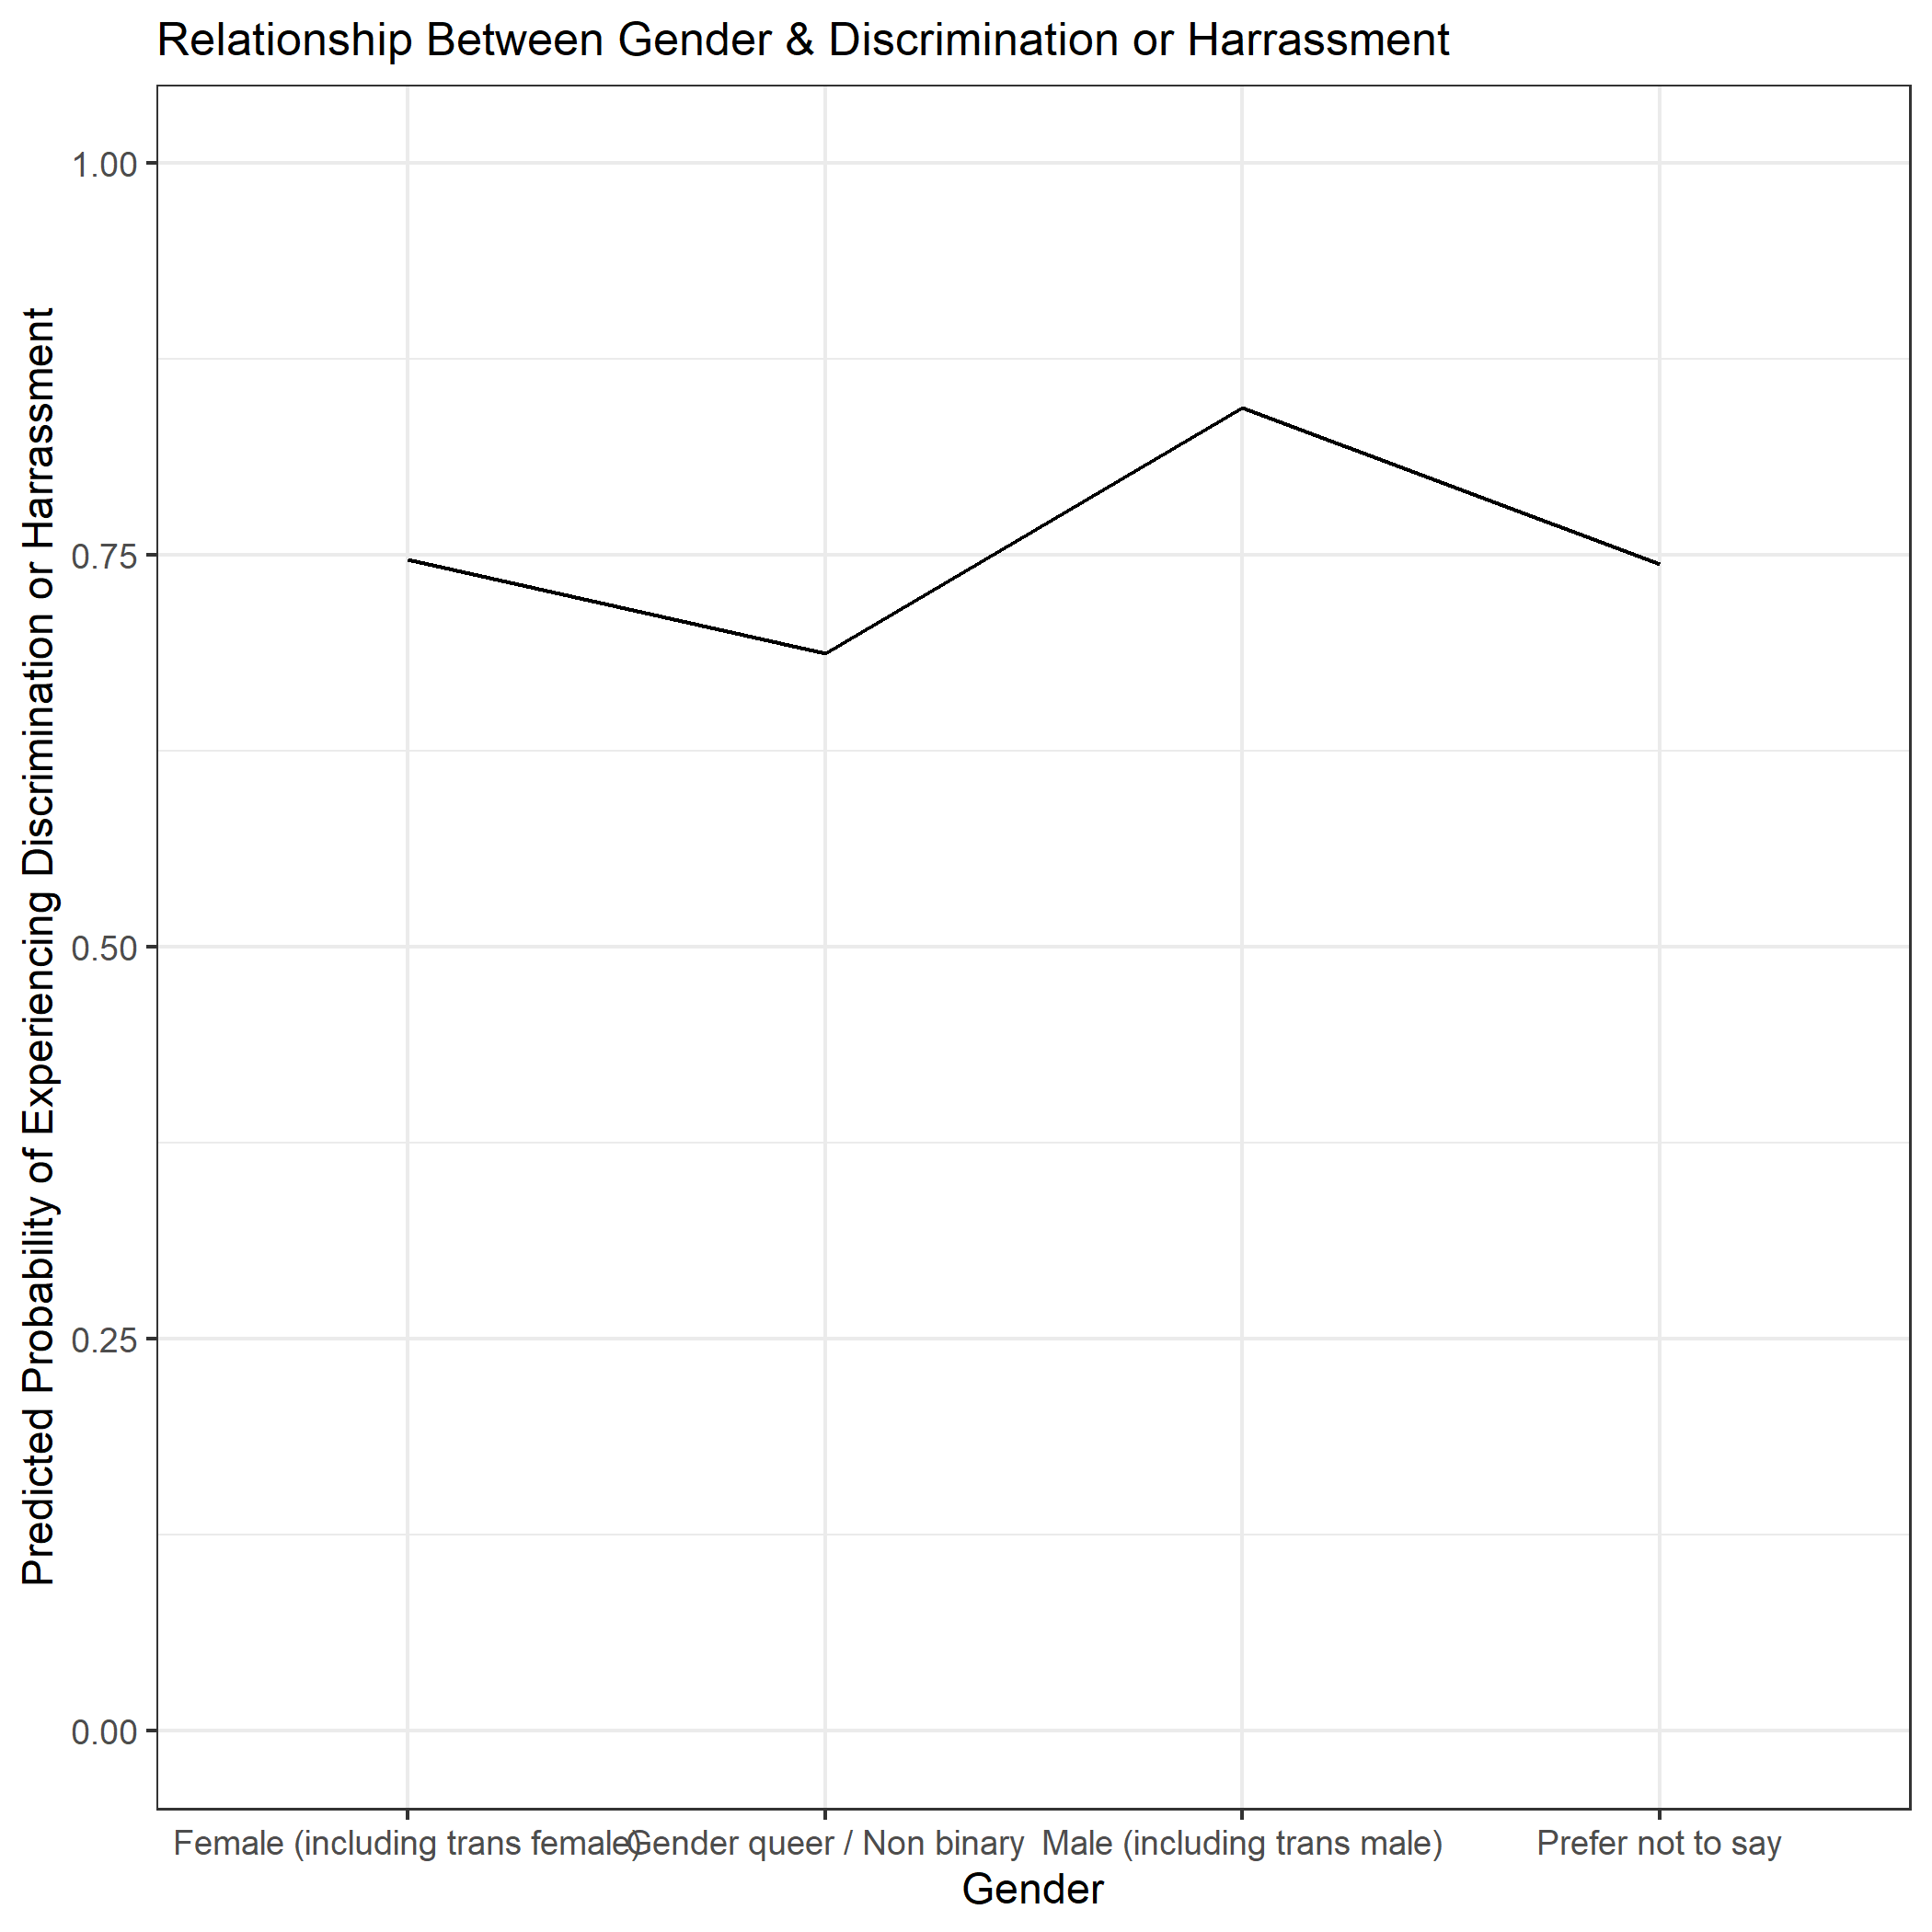
\includegraphics[width=29.17in]{C:/Users/iciar/OneDrive/Desktop/School/STAT547/group05/images/logisticregression7}

\hypertarget{discussion-and-conclusion}{%
\subsection{Discussion and Conclusion}\label{discussion-and-conclusion}}

\emph{Complete later.}

\hypertarget{references}{%
\subsection{References}\label{references}}

\emph{Complete later.}

\end{document}
